\documentclass[12pt,a4paper]{article}
\usepackage[utf8]{inputenc}
\usepackage[T1]{fontenc}
\usepackage[margin=2.5cm,headheight=16pt,headsep=18pt]{geometry}
\usepackage{graphicx}
\usepackage{fancyhdr}
\usepackage{booktabs}
\usepackage{tabularx}
\usepackage{multirow}
\usepackage{amsmath}
\usepackage{amssymb}
\usepackage{listings}
\usepackage{inconsolata}
\usepackage{caption}
\usepackage[section]{placeins}
\usepackage{needspace}
\usepackage{float}
\usepackage[normalem]{ulem}
\usepackage{url}
\usepackage{setspace}
\setstretch{1.15}
\usepackage[most]{tcolorbox}
% Hanya dua jenis kotak sorotan: Contoh dan Miskonsepsi umum.
\newtcolorbox{contoh}{enhanced,breakable,colback=blue!3,colframe=blue!45!black,boxrule=0.6pt,arc=2pt,left=6pt,right=6pt,top=4pt,bottom=4pt,fonttitle=\bfseries\small,title=Contoh,before skip=8pt,after skip=8pt}
\newtcolorbox{miskonsepsi}{enhanced,breakable,colback=orange!4,colframe=orange!60!black,boxrule=0.6pt,arc=2pt,left=6pt,right=6pt,top=4pt,bottom=4pt,fonttitle=\bfseries\small,title=Miskonsepsi umum,before skip=8pt,after skip=8pt}
\usepackage[hidelinks]{hyperref}
% Laporan dapat dikompilasi dari root repositori maupun dari folder docs.
\graphicspath{{docs/}{./}{../}}
\makeatletter
\def\input@path{{docs/}{./}}
\makeatother

\renewcommand{\contentsname}{Daftar Isi}
\renewcommand{\appendixname}{Lampiran}
\renewcommand{\tablename}{Tabel}
\renewcommand{\figurename}{Gambar}
\setcounter{tocdepth}{3}
\setlength{\parindent}{1.5em}
\setlength{\parskip}{0pt}
\lstset{language=Python,basicstyle=\ttfamily\footnotesize,keywordstyle=\bfseries,emphstyle=\bfseries,breaklines=true,frame=single,showstringspaces=false,columns=fullflexible,aboveskip=3pt,belowskip=3pt,floatplacement=htbp,float=htbp,float=true}
\makeatletter
\setlength{\@fpsep}{10pt}
\makeatother
\setlength{\textfloatsep}{10pt}
\setlength{\intextsep}{10pt}
\captionsetup{font=small,labelfont=bf,labelsep=period,skip=6pt}
\raggedbottom
\clubpenalty=10000
\widowpenalty=10000
\displaywidowpenalty=10000
\renewcommand{\topfraction}{0.9}
\renewcommand{\bottomfraction}{0.8}
\renewcommand{\textfraction}{0.08}
\renewcommand{\floatpagefraction}{0.75}
\AddToHook{cmd/subsection/before}{\FloatBarrier\Needspace{7\baselineskip}}
\AddToHook{cmd/subsubsection/before}{\FloatBarrier\Needspace{5\baselineskip}}
\renewcommand{\lstlistingname}{Cuplikan}
% Daftar pustaka tanpa nomor rujukan.
\makeatletter
\renewcommand{\@biblabel}[1]{}
\renewenvironment{thebibliography}[1]{\section*{\refname}\list{}{\leftmargin=1.5em\itemindent=-1.5em\itemsep=4pt\usecounter{enumiv}}\sloppy}{\endlist}
\makeatother
% Nama kolom panjang pada \texttt boleh dipenggal setelah garis bawah.
\DeclareRobustCommand{\_}{\textunderscore\allowbreak}
\setlength{\emergencystretch}{3em}

\pagestyle{fancy}
\fancyhf{}
\fancyhead[L]{IF3170 -- Inteligensi Artifisial}
\fancyhead[R]{\thepage}
\renewcommand{\headrulewidth}{0.4pt}
\renewcommand{\footrulewidth}{0pt}

% Kompilasi dari root repositori (jalankan dua kali agar daftar isi terbarui):
% pdflatex -output-directory=docs docs/laporan.tex
% Diagram bersumber dari docs/diagram/*.svg dan dikonversi ke PDF dengan:
% rsvg-convert -f pdf -o docs/diagram/<nama>.pdf docs/diagram/<nama>.svg
\begin{document}

\hypersetup{pageanchor=false}
\begin{titlepage}
    \centering
    {\Huge\bfseries Laporan Tugas Besar 2\par}
    \vspace{0.5cm}
    {\LARGE\scshape IF3170 Inteligensi Artifisial\par}
    \vspace{0.3cm}
    {\Large\scshape Prediksi Pembatalan Pemesanan Penginapan\par}
    \vspace{0.2cm}
    {\Large\scshape dengan Algoritma \textit{Supervised Learning}\par}
    \vspace{0.3cm}
    {\Large\scshape Tahun Akademik 2026--2027\par}
    \vfill
    % Logo dari situs resmi ITB:
    % https://itb.ac.id/assets/images/Logo%20ITB_COLOR_2026%404x.png
    
\includegraphics[width=7.5cm,keepaspectratio]{logo-itb.png}\par
    \vfill
    {\large\bfseries Disusun oleh:\par}
    \vspace{0.3cm}
    {\large Kelompok G02 -- nutellabear\par}
    \vspace{0.3cm}
    {\large Samuelson Dharmawan Tanuraharja -- 13524001\par}
    {\large Edward David Rumahorbo -- 13524036\par}
    {\large Narendra Dharma Wistara M. -- 13524044\par}
    {\large Reinhard Alfonzo Hutabarat -- 13524056\par}
    {\large Miguel Rangga Deardo Sinaga -- 13524069\par}
    \vfill
    {\large\scshape Laboratorium Inteligensi Artifisial\par}
    {\large\scshape Program Studi Teknik Informatika\par}
    {\large\scshape Sekolah Teknik Elektro dan Informatika\par}
    {\large\scshape Institut Teknologi Bandung\par}
\end{titlepage}

\pagenumbering{arabic}
\hypersetup{pageanchor=true}
{\small\linespread{0.92}\selectfont\tableofcontents}
\clearpage

\section{Deskripsi Persoalan}
\subsection{Latar Belakang}
Pembatalan pemesanan merupakan persoalan nyata dalam industri perhotelan. Kamar yang telah dipesan lalu dibatalkan mendekati tanggal kedatangan berpotensi kosong, sementara penjualan ulang kamar yang diperkirakan batal berisiko menimbulkan \textit{overbooking} apabila tamu ternyata tetap datang. Dalam skenario tugas ini, Ronaldo Hotel\texttrademark{} membutuhkan sistem cerdas berbasis pembelajaran mesin klasik untuk memperkirakan pemesanan yang akan dibatalkan, tanpa sumber daya komputasi besar seperti \textit{deep learning}.

Persoalan ini dimodelkan sebagai klasifikasi biner. Setiap pemesanan direpresentasikan oleh atribut seperti jumlah tamu, lama menginap, jarak hari pemesanan terhadap kedatangan, tarif, dan kanal pemesanan. Target \texttt{is\_canceled} bernilai 1 apabila pemesanan dibatalkan dan 0 apabila tidak.

\subsection{Rumusan Persoalan dan Tujuan}
Kelompok diminta mengimplementasikan lima algoritma \textit{supervised learning} secara \textit{from scratch}, yaitu KNN, DTL, \textit{logistic regression}, SVM, dan \textit{Naive Bayes}. Implementasi tersebut dibandingkan dengan pustaka \textit{scikit-learn}, harus dapat disimpan dan dimuat ulang, serta digunakan untuk minimal satu \textit{submission} Kaggle yang \textit{reproducible}. Tahap pengolahan data mencakup \textit{data cleaning}, \textit{data transformation}, \textit{feature selection}, \textit{dimensionality reduction}, serta \textit{modeling and validation}. \textit{Preprocessing} pada data latih dan data uji dilakukan terpisah, dan kedua data tidak boleh digabungkan.

Tujuan laporan ini adalah menjelaskan pemahaman terhadap dataset, langkah \textit{cleaning} dan \textit{preprocessing} beserta alasannya, implementasi setiap algoritma, serta hasil eksperimen dan perbandingannya. Selain itu, laporan ini membahas visualisasi pohon keputusan, video lintasan parameter \textit{logistic regression}, visualisasi bidang pemisah SVM, graf \textit{Naive Bayes}, algoritma optimasi model, dan \textit{cost-sensitive classification}.

\subsection{Deskripsi Dataset}
Dataset terdiri atas \path{train.csv} dengan 27.373 baris berlabel dan \path{test.csv} dengan 6.844 baris tanpa label. Selain kolom \texttt{id} dan target, terdapat 17 fitur: 14 fitur numerik dan 3 fitur kategorikal. Kolom \texttt{id} hanya berfungsi sebagai pengenal baris pada berkas pengumpulan dan tidak digunakan sebagai fitur. Tabel~\ref{tab:fitur} merangkum fitur tersebut beserta proporsi nilai hilang pada data latih.

\begin{table}[htbp]
    \centering
    \small
    \renewcommand{\arraystretch}{1.08}
    \begin{tabularx}{\textwidth}{@{}l l r X@{}}
        \toprule
        Fitur & Tipe & Hilang (\%) & Keterangan \\
        \midrule
        \texttt{num\_adults} & numerik & 2,96 & Jumlah tamu dewasa (0--4). \\
        \texttt{num\_children} & numerik & 11,09 & Jumlah anak (0--10). \\
        \texttt{weekend\_nights} & numerik & 0 & Jumlah malam akhir pekan. \\
        \texttt{weekday\_nights} & numerik & 0 & Jumlah malam hari kerja. \\
        \texttt{meal\_package} & kategorikal & 6,43 & Paket makan: Breakfast, Room Only, Half Board, Full Board. \\
        \texttt{needs\_parking} & numerik & 3,95 & Kebutuhan parkir (0/1). \\
        \texttt{room\_category} & kategorikal & 3,66 & Tipe kamar A--G. \\
        \texttt{days\_before\_arrival} & numerik & 4,10 & Selisih hari pemesanan dan kedatangan (0--448). \\
        \texttt{arrival\_year} & numerik & 0 & Tahun kedatangan (2023 atau 2024). \\
        \texttt{arrival\_month} & numerik & 0 & Bulan kedatangan. \\
        \texttt{arrival\_day} & numerik & 0 & Tanggal kedatangan. \\
        \texttt{booking\_channel} & kategorikal & 0 & Kanal: Online Travel Agent, Offline Agent, Corporate, Complimentary, Airline. \\
        \texttt{is\_returning\_guest} & numerik & 0 & Tamu yang pernah menginap (0/1). \\
        \texttt{prior\_cancellations} & numerik & 0 & Jumlah pembatalan sebelumnya. \\
        \texttt{prior\_completed\_bookings} & numerik & 0 & Jumlah pemesanan sebelumnya yang tidak dibatalkan. \\
        \texttt{nightly\_rate\_idr} & numerik & 7,45 & Tarif per malam dalam rupiah. \\
        \texttt{special\_requests} & numerik & 9,13 & Jumlah permintaan khusus (0--5). \\
        \bottomrule
    \end{tabularx}
    \caption{Fitur dataset dan proporsi nilai hilang pada \texttt{train.csv}.}
    \label{tab:fitur}
\end{table}

\subsection{Pemahaman Data}\label{sec:eda}
Pemahaman data dimulai dari distribusi kelas. Sebanyak 32,77\% pemesanan pada data latih berlabel batal. Dataset tidak seimbang secara ekstrem, tetapi tebakan yang selalu memilih kelas mayoritas sudah memperoleh akurasi 0,6723 pada data validasi. Angka ini menjadi baseline yang harus dilampaui setiap model.

Dari sisi kualitas data, delapan fitur memiliki nilai hilang, dan 10.737 baris latih memiliki sedikitnya satu nilai hilang. Karena jumlah tersebut mencapai 39\% data latih, penghapusan baris akan membuang terlalu banyak informasi sehingga imputasi atau penanganan nilai hilang di dalam model lebih tepat. Pemeriksaan pada seluruh \path{train.csv} juga menemukan 66 salinan duplikat berdasarkan fitur, dua kelompok duplikat dengan label bertentangan, dan 64 baris tanpa malam menginap. Tidak ada baris tanpa tamu. Aturan IQR menandai cukup banyak pencilan, misalnya 916 baris pada \texttt{days\_before\_arrival} dan 1.144 baris pada \texttt{nightly\_rate\_idr}.

Hubungan fitur dengan target terlihat dari korelasi. Korelasi linear terkuat terhadap target dimiliki \texttt{days\_before\_arrival} ($+0{,}440$) dan \texttt{special\_requests} ($-0{,}258$), diikuti \texttt{arrival\_year} ($+0{,}180$) dan \texttt{nightly\_rate\_idr} ($+0{,}134$). Artinya, pemesanan yang dibuat jauh hari sebelum kedatangan lebih sering dibatalkan, sedangkan tamu yang mengajukan permintaan khusus cenderung datang. Gambar~\ref{fig:eda-kategori} menunjukkan rasio pembatalan per kategori. Kanal Corporate dan Complimentary jauh lebih jarang batal dibanding rata-rata, sedangkan paket Half Board dan kamar Type A lebih sering batal.

\begin{figure}[htbp]
    \centering
    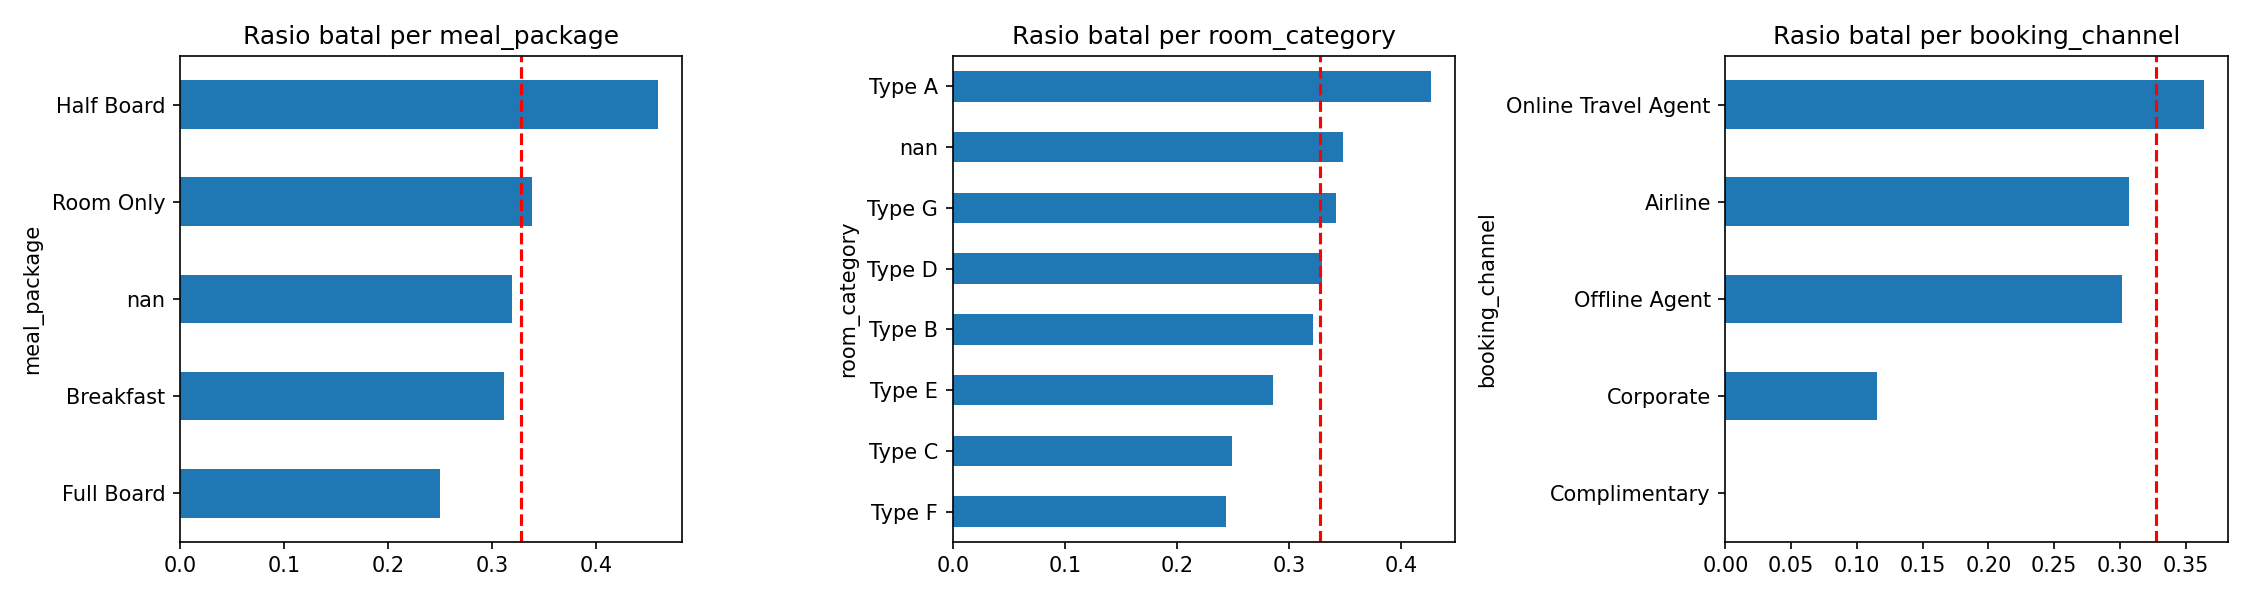
\includegraphics[width=\textwidth]{output/eda/cancel_rate_categorical.png}
    \caption{Rasio pembatalan per kategori. Garis merah menandai rasio pembatalan keseluruhan.}
    \label{fig:eda-kategori}
\end{figure}

\begin{figure}[htbp]
    \centering
    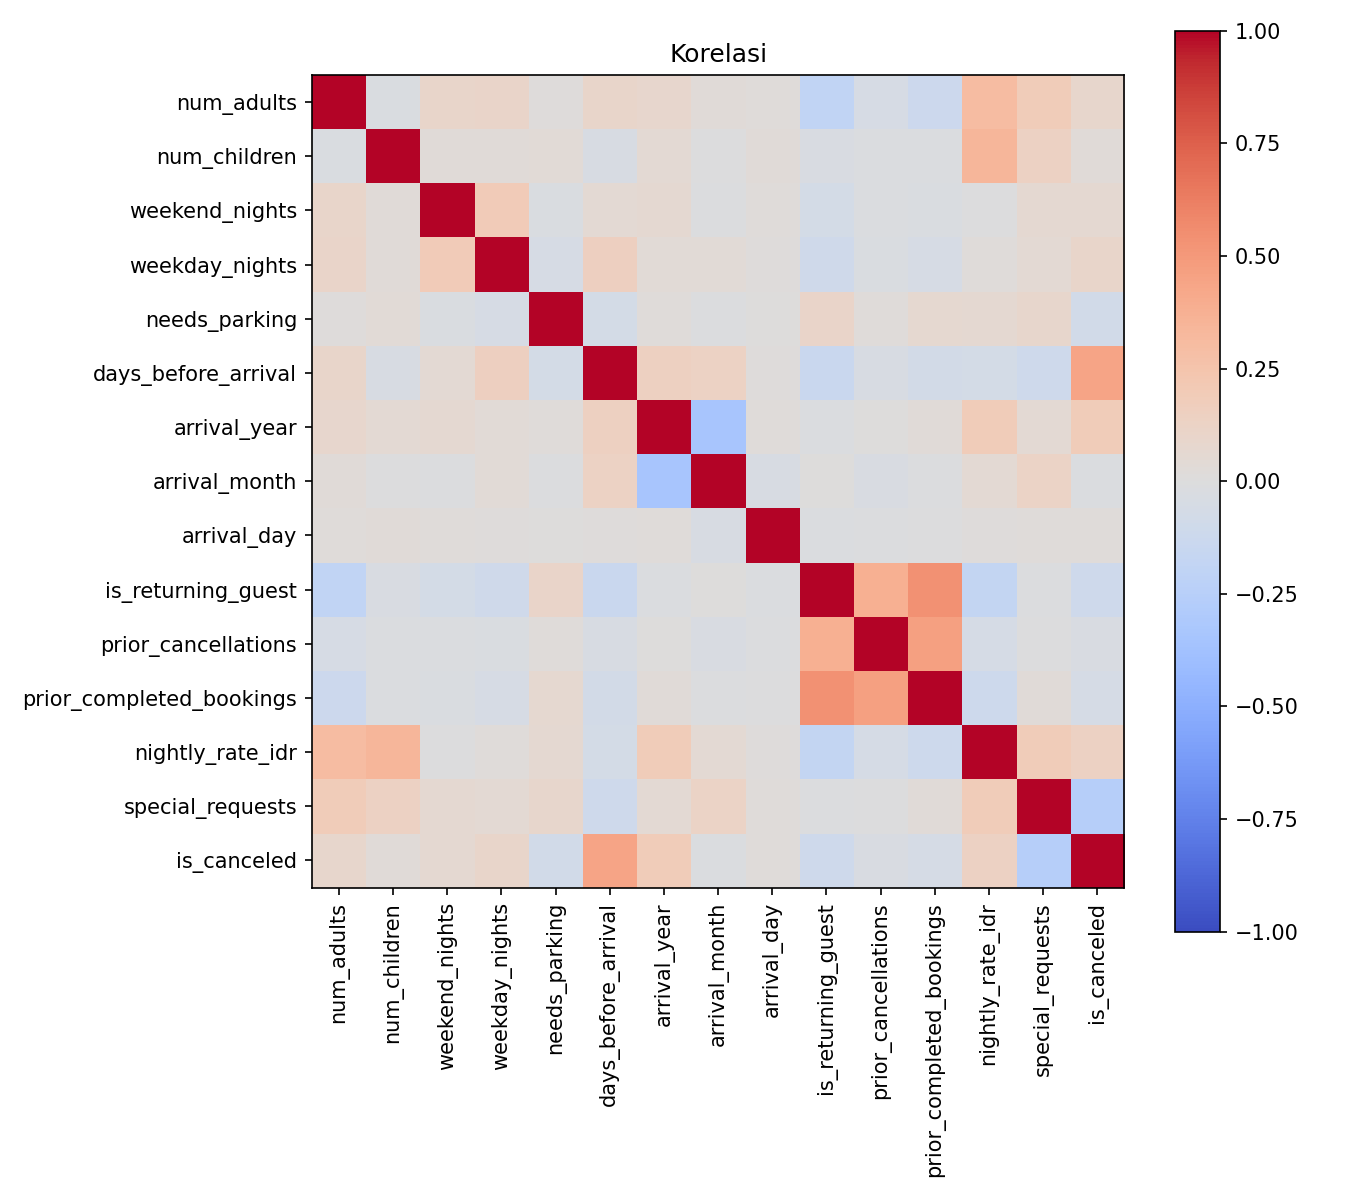
\includegraphics[width=0.72\textwidth]{output/eda/correlation.png}
    \caption{Matriks korelasi Pearson antarfitur numerik dan target.}
    \label{fig:eda-korelasi}
\end{figure}

Data latih dan data uji juga dibandingkan untuk mendeteksi pergeseran distribusi. Statistik Kolmogorov--Smirnov untuk fitur numerik dan \textit{total variation distance} untuk fitur kategorikal seluruhnya di bawah 0,015. Proporsi nilai hilang pada data uji juga mendekati data latih, misalnya 10,91\% berbanding 11,09\% untuk \texttt{num\_children}, dan tidak ada kategori baru pada data uji. Dengan demikian, distribusi data uji dapat dianggap sama dengan data latih, sehingga skor validasi lokal dapat digunakan sebagai perkiraan kinerja pada Kaggle. Pemeriksaan ini hanya membandingkan distribusi fitur dan tidak menggunakan label uji.

\clearpage
\section{Dasar Teori}
\subsection{\textit{Supervised Learning} dan Klasifikasi}
\textit{Supervised learning} adalah paradigma pembelajaran mesin yang mempelajari fungsi pemetaan $h:\mathcal{X}\rightarrow\mathcal{Y}$ dari kumpulan contoh berlabel $D=\{(\mathbf{x}_i,y_i)\}_{i=1}^{n}$. Setiap $\mathbf{x}_i$ adalah vektor fitur, sedangkan $y_i$ adalah keluaran yang diketahui. Apabila $\mathcal{Y}$ berupa himpunan kelas berhingga, persoalannya disebut klasifikasi. Pada tugas ini $\mathcal{Y}=\{0,1\}$ sehingga persoalannya merupakan klasifikasi biner.

Tujuan pembelajaran bukan menghafal data latih, melainkan memperoleh hipotesis yang menggeneralisasi dengan baik pada data yang belum pernah dilihat. Hipotesis yang terlalu sederhana menghasilkan \textit{underfitting}, yaitu galat besar pada data latih maupun data baru. Sebaliknya, hipotesis yang terlalu kompleks dapat mengikuti derau pada data latih sehingga mengalami \textit{overfitting}. Oleh sebab itu, kinerja model selalu diukur pada data yang terpisah dari data latih, dan kompleksitas model dikendalikan melalui \textit{hyperparameter}, regularisasi, atau pemangkasan.

Sebagian besar model pada tugas ini menghasilkan skor peluang $\hat{p}(\mathbf{x})=P(y=1\mid\mathbf{x})$. Label diperoleh dengan membandingkan skor tersebut terhadap ambang $\tau$, yaitu $\hat{y}=\mathbb{1}[\hat{p}(\mathbf{x})\geq\tau]$. Ambang baku adalah $\tau=0{,}5$, tetapi ambang dapat diubah ketika biaya kesalahan tidak simetris, sebagaimana dibahas pada Subbab~\ref{sec:teori-cost}.

\subsection{CRISP-DM, \textit{Data Understanding}, dan \textit{Data Preparation}}
\textit{Cross-Industry Standard Process for Data Mining} (CRISP-DM) membagi proyek data menjadi enam fase: \textit{business understanding}, \textit{data understanding}, \textit{data preparation}, \textit{modeling}, \textit{evaluation}, dan \textit{deployment}. Fase-fase tersebut bersifat iteratif. Temuan pada pemodelan sering memaksa kembali ke tahap persiapan data. Templat notebook tugas ini mengikuti urutan yang sama, mulai dari pemahaman data hingga pengumpulan prediksi.

\textit{Data understanding} mencakup deskripsi data (ukuran, tipe, dan arti kolom), eksplorasi (distribusi dan hubungan fitur dengan target), serta verifikasi kualitas (nilai hilang, duplikat, nilai tidak valid, dan pencilan). Hasil fase ini menentukan langkah persiapan yang diperlukan.

\textit{Data preparation} mengubah data mentah menjadi representasi yang dapat diproses algoritma. Langkah utamanya adalah sebagai berikut.
\begin{enumerate}
    \setlength{\itemsep}{0pt}
    \item \textbf{\textit{Data cleaning}}\\
    Nilai hilang dapat dihapus atau diimputasi, misalnya dengan median untuk fitur numerik dan modus untuk fitur kategorikal. Median lebih tahan terhadap pencilan daripada rata-rata. Baris duplikat dan baris yang melanggar aturan domain juga ditangani pada tahap ini. Pencilan dapat dideteksi dengan aturan IQR, yaitu nilai di luar $[Q_1-1{,}5\,\mathrm{IQR},\,Q_3+1{,}5\,\mathrm{IQR}]$, lalu dipotong (\textit{clipping}) ke persentil tertentu.
    \item \textbf{\textit{Data transformation}}\\
    Fitur kategorikal diubah menjadi angka melalui \textit{one-hot encoding}, yaitu satu kolom biner untuk setiap kategori. Fitur numerik diskalakan agar setara, misalnya dengan standardisasi $z=(x-\mu)/\sigma$ atau normalisasi min-max $x'=(x-x_{\min})/(x_{\max}-x_{\min})$. Penskalaan penting bagi model berbasis jarak dan gradien, karena fitur bernilai besar akan mendominasi jarak maupun langkah optimasi.
    \item \textbf{\textit{Feature construction} dan \textit{feature selection}}\\
    Fitur turunan dapat merangkum beberapa kolom menjadi informasi yang lebih bermakna. Pemilihan fitur membuang atribut yang kurang relevan. Salah satu ukurannya adalah \textit{mutual information} $I(X;Y)=\sum_{x,y}p(x,y)\log_2\frac{p(x,y)}{p(x)p(y)}$, yang bernilai nol apabila fitur dan target saling bebas.
    \item \textbf{\textit{Dimensionality reduction}}\\
    \textit{Principal Component Analysis} (PCA) memproyeksikan data ke arah vektor eigen matriks kovarians dengan ragam terbesar. Jumlah komponen dipilih agar proporsi ragam kumulatif melewati batas tertentu, misalnya 95\%.
    \item \textbf{Penanganan ketidakseimbangan kelas}\\
    \textit{Random oversampling} menyalin sampel kelas minoritas secara acak hingga jumlah kedua kelas seimbang. Teknik ini hanya boleh diterapkan pada data latih.
\end{enumerate}

Prinsip terpenting dalam persiapan data adalah mencegah \textit{data leakage}. Seluruh statistik yang dipelajari dari data, seperti median imputasi, batas \textit{clipping}, kategori \textit{encoder}, rata-rata dan simpangan baku \textit{scaler}, skor seleksi fitur, serta komponen PCA, harus di-\textit{fit} hanya pada data latih. Data validasi dan data uji cukup di-\textit{transform}. Jika aturan ini dilanggar, skor validasi menjadi terlalu optimis dan tidak mencerminkan kinerja pada data baru.

\subsection{\textit{k-Nearest Neighbors}}
\textit{k-Nearest Neighbors} (KNN) adalah metode \textit{instance-based} atau \textit{lazy learning}. Pada fase pelatihan, KNN hanya menyimpan seluruh data latih. Ketika menerima titik kueri $\mathbf{x}_q$, KNN menghitung jarak ke setiap data latih, mengambil $k$ tetangga terdekat $N_k(\mathbf{x}_q)$, lalu menentukan kelas berdasarkan suara tetangga tersebut. Gambar~\ref{fig:teori-knn} mengilustrasikan proses ini.

Jarak yang umum digunakan adalah keluarga Minkowski orde $p$:
\begin{equation}
    d_p(\mathbf{a},\mathbf{b})=\left(\sum_{j=1}^{m}|a_j-b_j|^{p}\right)^{1/p}.
    \label{eq:minkowski}
\end{equation}
Nilai $p=1$ menghasilkan jarak Manhattan, sedangkan $p=2$ menghasilkan jarak Euclidean. Untuk klasifikasi biner, peluang kelas positif diperkirakan dari proporsi tetangga positif. Dengan pembobotan jarak, tetangga yang lebih dekat diberi pengaruh lebih besar:
\begin{equation}
    \hat{p}(\mathbf{x}_q)=\frac{\sum_{i\in N_k(\mathbf{x}_q)}w_i\,y_i}{\sum_{i\in N_k(\mathbf{x}_q)}w_i},\qquad
    w_i=\begin{cases}1 & \text{(\textit{uniform})},\\ 1/d(\mathbf{x}_q,\mathbf{x}_i) & \text{(\textit{distance})}.\end{cases}
    \label{eq:knn-proba}
\end{equation}

Nilai $k$ mengatur keseimbangan bias dan variansi. Nilai $k$ kecil membuat batas keputusan sangat lokal dan peka derau, sedangkan nilai $k$ besar menghaluskan batas keputusan tetapi dapat mengaburkan pola lokal. Karena seluruh perhitungan terjadi saat prediksi, kompleksitas waktu prediksi naif adalah $O(n\,m)$ untuk setiap kueri, dengan $n$ jumlah data latih dan $m$ jumlah fitur. KNN juga sangat bergantung pada skala fitur dan rentan terhadap \textit{curse of dimensionality}, yaitu kondisi ketika jarak antartitik menjadi kurang informatif pada dimensi tinggi.

\begin{figure}[htbp]
    \centering
    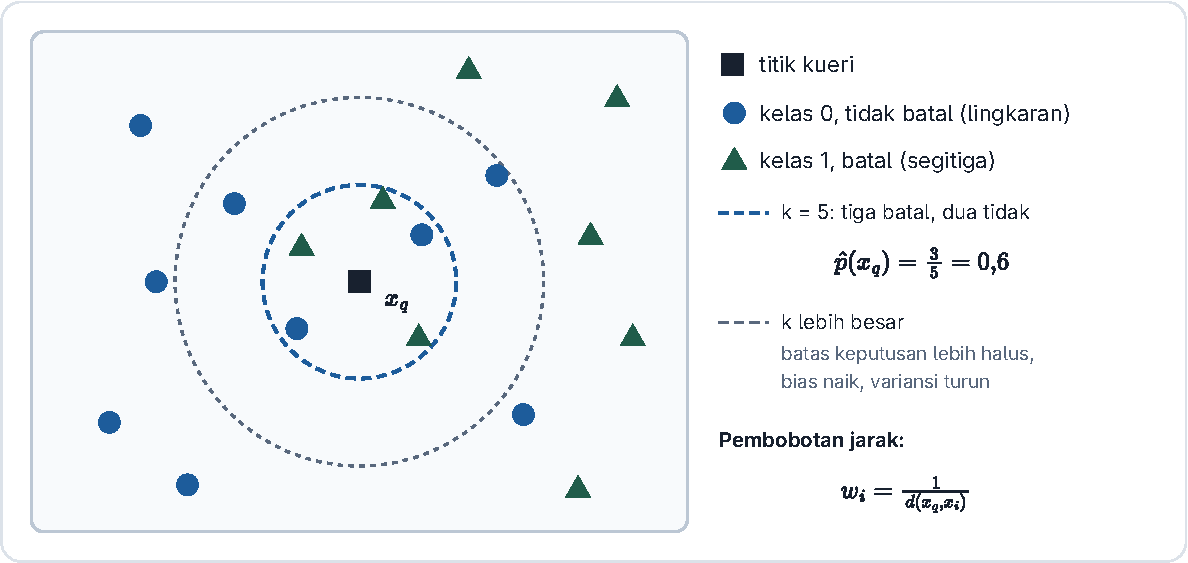
\includegraphics[width=0.82\textwidth]{diagram/knn.pdf}
    \caption{Ilustrasi KNN: kelas titik kueri ditentukan oleh $k$ tetangga terdekat. Jari-jari lingkaran bergantung pada nilai $k$.}
    \label{fig:teori-knn}
\end{figure}

\subsection{\textit{Decision Tree Learning}}
\textit{Decision Tree Learning} (DTL) membangun pohon keputusan secara \textit{top-down} dan rakus (\textit{greedy}). Setiap simpul internal menguji satu atribut, setiap cabang mewakili hasil uji, dan setiap daun menyimpan distribusi kelas. Algoritma dasar ID3 memilih atribut yang paling memurnikan data pada setiap simpul, lalu mengulang proses secara rekursif pada setiap cabang hingga data murni atau atribut habis.

\subsubsection{Entropi, \textit{Information Gain}, dan \textit{Gain Ratio}}
Ketidakmurnian himpunan $S$ diukur dengan entropi
\begin{equation}
    H(S)=-\sum_{c}p_c\log_2 p_c,
    \label{eq:entropy}
\end{equation}
dengan $p_c$ proporsi kelas $c$ pada $S$. Entropi bernilai nol untuk himpunan murni dan bernilai maksimum satu bit untuk dua kelas yang seimbang. Pengurangan entropi setelah memecah $S$ menurut atribut $A$ disebut \textit{information gain}:
\begin{equation}
    \mathrm{Gain}(S,A)=H(S)-\sum_{v\in\mathrm{Values}(A)}\frac{|S_v|}{|S|}H(S_v).
    \label{eq:gain}
\end{equation}
\textit{Information gain} cenderung memilih atribut dengan banyak nilai, karena atribut seperti itu memecah data menjadi banyak subset kecil yang mudah murni. C4.5 mengoreksi bias tersebut dengan \textit{gain ratio}:
\begin{equation}
    \mathrm{SplitInfo}(S,A)=-\sum_{v}\frac{|S_v|}{|S|}\log_2\frac{|S_v|}{|S|},\qquad
    \mathrm{GainRatio}(S,A)=\frac{\mathrm{Gain}(S,A)}{\mathrm{SplitInfo}(S,A)}.
    \label{eq:gain-ratio}
\end{equation}
Karena \textit{gain ratio} dapat membesar secara semu ketika $\mathrm{SplitInfo}$ mendekati nol, C4.5 hanya membandingkan \textit{gain ratio} di antara atribut yang \textit{information gain}-nya minimal sebesar rata-rata \textit{gain} seluruh kandidat.

\begin{contoh}
Sebagai ilustrasi, himpunan $S$ berisi 10 pemesanan: 4 batal dan 6 tidak batal, sehingga $H(S)=-(0{,}4\log_2 0{,}4+0{,}6\log_2 0{,}6)=0{,}9710$. Atribut biner $A$ memecah $S$ menjadi dua cabang berisi 5 sampel. Cabang pertama memuat 4 batal dan 1 tidak batal dengan $H=0{,}7219$, sedangkan cabang kedua murni tidak batal dengan $H=0$. Dengan demikian,
\[
\mathrm{Gain}(S,A)=0{,}9710-\tfrac{5}{10}(0{,}7219)-\tfrac{5}{10}(0)=0{,}6100,\qquad \mathrm{SplitInfo}(S,A)=1,
\]
sehingga $\mathrm{GainRatio}(S,A)=0{,}6100$. Karena pemecahannya seimbang, \textit{split information} bernilai satu dan \textit{gain ratio} sama dengan \textit{gain}. Atribut yang memecah data menjadi banyak cabang kecil akan memiliki \textit{split information} lebih besar dan karenanya dihukum.
\end{contoh}

CART memakai ukuran lain, yaitu indeks Gini $G(S)=1-\sum_c p_c^2$, dan selalu membentuk pohon biner. Tabel~\ref{tab:varian-dtl} merangkum perbedaan ketiga varian tersebut.

\begin{table}[htbp]
    \centering
    \small
    \renewcommand{\arraystretch}{1.15}
    \begin{tabularx}{\textwidth}{@{}lXXX@{}}
        \toprule
        Aspek & ID3 & C4.5 & CART \\
        \midrule
        Ukuran pemisahan & \textit{Information gain} & \textit{Gain ratio} & Indeks Gini \\
        Atribut numerik & Tidak langsung & Ambang biner $A\leq t$ & Ambang biner $A\leq t$ \\
        Atribut kategorikal & Cabang per nilai & Cabang per nilai & Pemisahan biner himpunan nilai \\
        Nilai hilang & Tidak ditangani & Bobot pecahan & \textit{Surrogate split} \\
        Pemangkasan & Tidak ada & \textit{Error-based pruning} & \textit{Cost-complexity pruning} \\
        \bottomrule
    \end{tabularx}
    \caption{Perbandingan varian DTL.}
    \label{tab:varian-dtl}
\end{table}

\subsubsection{Atribut Kontinu dan Nilai Hilang}
Atribut kontinu ditangani dengan mencari ambang $t$ sehingga data terbagi menjadi $A\leq t$ dan $A>t$. Kandidat ambang cukup diambil dari titik tengah dua nilai berurutan yang berbeda setelah data diurutkan, karena ambang optimum untuk ukuran berbasis entropi selalu berada di antara dua nilai seperti itu.

Untuk nilai hilang, C4.5 menghitung \textit{gain} hanya pada sampel yang nilainya diketahui, lalu mengalikannya dengan proporsi sampel yang diketahui. Saat pemecahan, sampel dengan nilai hilang dikirim ke semua cabang dengan bobot pecahan sebanding dengan proporsi sampel diketahui pada cabang tersebut. Saat prediksi, data uji yang nilainya hilang menelusuri seluruh cabang, dan distribusi kelas dari daun-daun yang dicapai digabung sesuai bobot cabangnya. Gambar~\ref{fig:teori-dtree} memperlihatkan mekanisme ini.

\begin{figure}[htbp]
    \centering
    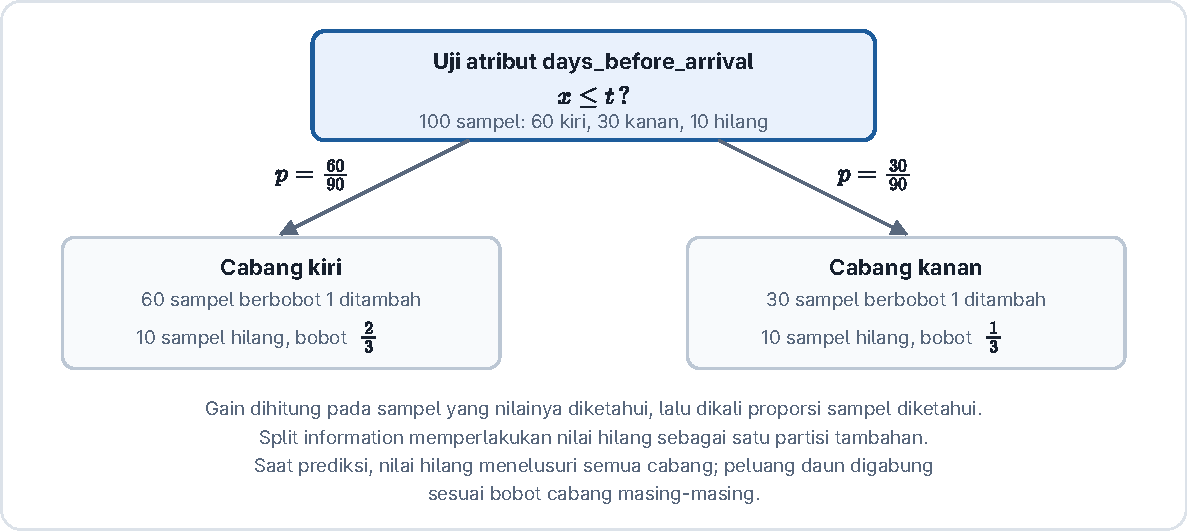
\includegraphics[width=0.82\textwidth]{diagram/dtree.pdf}
    \caption{Distribusi bobot pecahan untuk sampel bernilai hilang pada C4.5.}
    \label{fig:teori-dtree}
\end{figure}

\subsubsection{\textit{Overfitting} dan Pemangkasan}
Pohon yang dibiarkan tumbuh hingga murni cenderung \textit{overfit}, karena daun-daun kecil mencerminkan derau. Pertumbuhan dapat dihentikan lebih awal (\textit{pre-pruning}) melalui batas kedalaman, jumlah sampel minimum, atau \textit{gain} minimum. Pohon juga dapat dipangkas setelah dibangun (\textit{post-pruning}). \textit{Cost-complexity pruning} pada CART meminimalkan
\begin{equation}
    R_\alpha(T)=R(T)+\alpha\,|\widetilde{T}|,
    \label{eq:ccp}
\end{equation}
dengan $R(T)$ galat klasifikasi pohon, $|\widetilde{T}|$ jumlah daun, dan $\alpha\geq0$ harga setiap daun tambahan. Subpohon diganti daun apabila galatnya sebagai daun ditambah $\alpha$ tidak lebih besar daripada jumlah biaya subpohon tersebut. Nilai $\alpha$ dipilih melalui validasi silang.

\subsection{\textit{Logistic Regression}}
\textit{Logistic regression} memodelkan peluang kelas positif dengan fungsi sigmoid dari kombinasi linear fitur:
\begin{equation}
    \hat{p}(\mathbf{x})=\sigma(z)=\frac{1}{1+e^{-z}},\qquad z=\mathbf{w}^\top\mathbf{x}+b.
    \label{eq:sigmoid}
\end{equation}
Batas keputusan $\hat{p}=0{,}5$ setara dengan $z=0$, sehingga model ini menghasilkan hyperplane linear di ruang fitur. Parameter diperoleh dengan memaksimalkan \textit{likelihood}, atau secara setara meminimalkan rata-rata \textit{log-loss} (\textit{binary cross-entropy}):
\begin{equation}
    \mathcal{L}(\mathbf{w},b)=-\frac{1}{n}\sum_{i=1}^{n}\Big[y_i\log\hat{p}_i+(1-y_i)\log(1-\hat{p}_i)\Big].
    \label{eq:logloss}
\end{equation}
Fungsi ini konveks, dan gradiennya berbentuk sederhana:
\begin{equation}
    \nabla_{\mathbf{w}}\mathcal{L}=\frac{1}{n}\sum_{i=1}^{n}(\hat{p}_i-y_i)\,\mathbf{x}_i,\qquad
    \frac{\partial\mathcal{L}}{\partial b}=\frac{1}{n}\sum_{i=1}^{n}(\hat{p}_i-y_i).
    \label{eq:lr-grad}
\end{equation}
\textit{Gradient descent} memperbarui parameter dengan $\mathbf{w}\leftarrow\mathbf{w}-\eta\nabla_{\mathbf{w}}\mathcal{L}$ dengan laju belajar $\eta$. Varian \textit{stochastic} atau \textit{mini-batch} menghitung gradien dari sebagian data pada setiap langkah sehingga pembaruan lebih sering dilakukan. Dalam formulasi \textit{gradient ascent}, kuliah memaksimalkan \textit{log-likelihood}. Kedua formulasi menghasilkan pembaruan yang sama dengan tanda berlawanan.

\subsubsection{Regularisasi}
Regularisasi menambahkan penalti $R(\mathbf{w})$ ke fungsi tujuan, $J=\mathcal{L}+R(\mathbf{w})$, untuk mengendalikan besar bobot dan mengurangi \textit{overfitting}. Bias $b$ umumnya tidak diregularisasi. Tiga bentuk penalti yang diminta adalah
\begin{equation}
    R_{L1}=\alpha\|\mathbf{w}\|_1,\qquad
    R_{L2}=\frac{\alpha}{2}\|\mathbf{w}\|_2^2,\qquad
    R_{EN}=\alpha\left(\rho\|\mathbf{w}\|_1+\frac{1-\rho}{2}\|\mathbf{w}\|_2^2\right),
    \label{eq:reg}
\end{equation}
dengan $\rho$ porsi L1 pada Elastic Net. Penalti L2 (\textit{ridge}) mengecilkan seluruh bobot secara proporsional tanpa membuatnya tepat nol. Penalti L1 (\textit{lasso}) mendorong sebagian bobot menjadi tepat nol sehingga sekaligus melakukan seleksi fitur. Elastic Net menggabungkan keduanya, sehingga tetap menghasilkan bobot jarang tetapi lebih stabil ketika fitur saling berkorelasi. Gambar~\ref{fig:teori-lr} menunjukkan alasan geometrisnya. Kontur \textit{loss} lebih mungkin menyentuh daerah L1 pada sudutnya, yaitu titik dengan salah satu bobot bernilai nol.

Penalti L1 tidak terdiferensialkan di nol. Salah satu cara menanganinya adalah \textit{proximal gradient}. Pada metode ini, langkah gradien dilakukan pada bagian yang mulus, lalu bobot dilewatkan ke operator \textit{soft-threshold}
\begin{equation}
    \mathrm{prox}_{\eta\lambda}(w)=\mathrm{sign}(w)\max(|w|-\eta\lambda,\,0).
    \label{eq:soft-threshold}
\end{equation}
Operator ini menggeser bobot ke arah nol sebesar $\eta\lambda$ dan menetapkannya tepat nol apabila besarnya lebih kecil daripada ambang tersebut.

\begin{figure}[htbp]
    \centering
    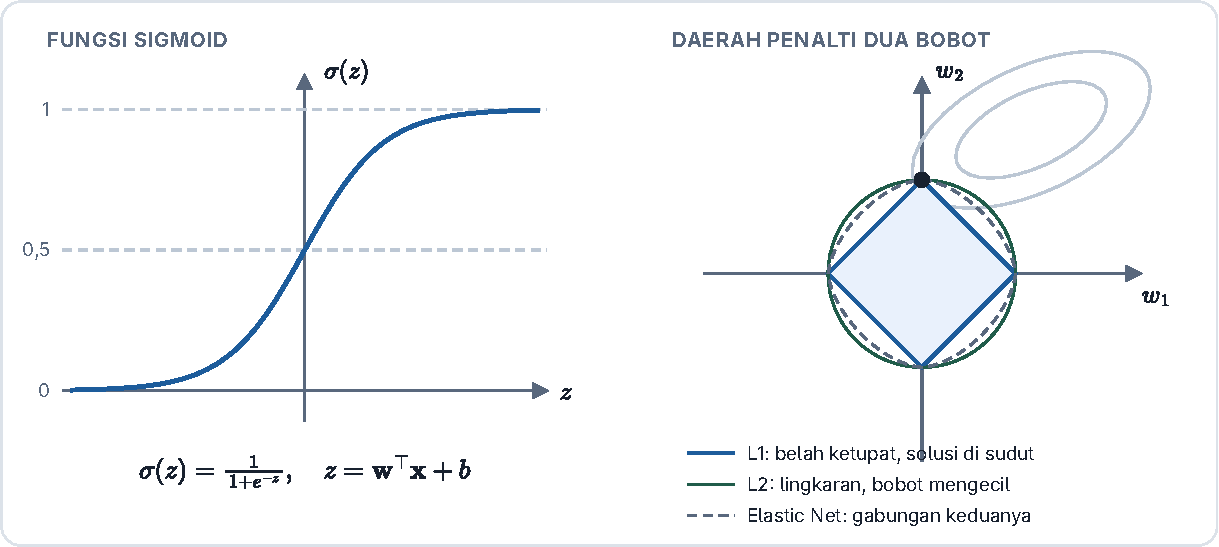
\includegraphics[width=0.92\textwidth]{diagram/logreg.pdf}
    \caption{Fungsi sigmoid (kiri) serta daerah batasan penalti L1, L2, dan Elastic Net pada dua bobot beserta kontur \textit{loss} (kanan).}
    \label{fig:teori-lr}
\end{figure}

\subsection{\textit{Support Vector Machine}}
\textit{Support Vector Machine} (SVM) mencari hyperplane $\mathbf{w}^\top\mathbf{x}+b=0$ yang memisahkan dua kelas dengan margin terbesar. Dengan label $y_i\in\{-1,+1\}$, lebar margin adalah $2/\|\mathbf{w}\|$, sehingga pada data yang terpisah linear persoalannya adalah meminimalkan $\frac{1}{2}\|\mathbf{w}\|^2$ dengan syarat $y_i(\mathbf{w}^\top\mathbf{x}_i+b)\geq1$. Data nyata jarang terpisah sempurna, sehingga \textit{soft-margin} SVM menambahkan variabel \textit{slack} $\xi_i\geq0$:
\begin{equation}
    \min_{\mathbf{w},b,\boldsymbol{\xi}}\ \frac{1}{2}\|\mathbf{w}\|^2+C\sum_{i=1}^{n}\xi_i
    \quad\text{dengan}\quad y_i(\mathbf{w}^\top\mathbf{x}_i+b)\geq1-\xi_i.
    \label{eq:svm-primal}
\end{equation}
Parameter $C$ mengatur kompromi antara margin lebar dan banyaknya pelanggaran. Bentuk dual persoalan ini adalah
\begin{equation}
    \max_{\boldsymbol{\alpha}}\ \sum_{i}\alpha_i-\frac{1}{2}\sum_{i,j}\alpha_i\alpha_j y_i y_j K(\mathbf{x}_i,\mathbf{x}_j)
    \quad\text{dengan}\quad 0\leq\alpha_i\leq C,\ \sum_i\alpha_i y_i=0,
    \label{eq:svm-dual}
\end{equation}
dan fungsi keputusan $f(\mathbf{x})=\sum_{i}\alpha_i y_i K(\mathbf{x}_i,\mathbf{x})+b$. Hanya sampel dengan $\alpha_i>0$ yang memengaruhi $f$. Sampel tersebut disebut \textit{support vector} dan berada pada atau di dalam margin. Gambar~\ref{fig:teori-svm} merangkum konsep margin dan kernel.

\begin{figure}[htbp]
    \centering
    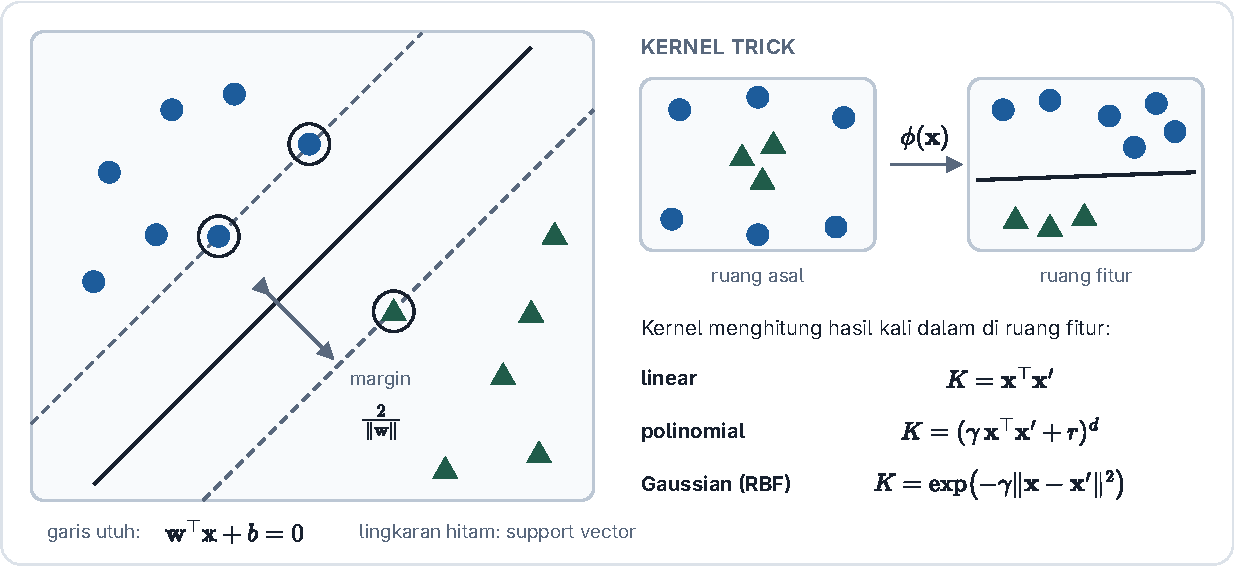
\includegraphics[width=0.95\textwidth]{diagram/svm.pdf}
    \caption{Hyperplane pemisah, margin, dan \textit{support vector} (kiri) serta pemetaan kernel yang membuat data tidak terpisah linear menjadi terpisah di ruang fitur (kanan).}
    \label{fig:teori-svm}
\end{figure}

\subsubsection{Kernel}
Bentuk dual hanya memerlukan hasil kali dalam antarsampel. Fungsi kernel $K(\mathbf{x},\mathbf{x}')=\phi(\mathbf{x})^\top\phi(\mathbf{x}')$ menghitung hasil kali dalam di ruang fitur berdimensi tinggi tanpa membentuk $\phi$ secara eksplisit. Teknik ini disebut \textit{kernel trick}. Tiga kernel yang diminta adalah
\begin{equation}
    K_{\text{lin}}=\mathbf{x}^\top\mathbf{x}',\qquad
    K_{\text{poly}}=(\gamma\,\mathbf{x}^\top\mathbf{x}'+r)^d,\qquad
    K_{\text{RBF}}=\exp\!\left(-\gamma\|\mathbf{x}-\mathbf{x}'\|^2\right).
    \label{eq:kernels}
\end{equation}
Kernel Gaussian (RBF) setara dengan ruang fitur berdimensi tak hingga. Nilai $\gamma$ yang besar membuat pengaruh setiap \textit{support vector} sangat lokal sehingga batas keputusan berliku, sedangkan $\gamma$ kecil menghasilkan batas yang lebih halus.

\subsubsection{\textit{Sequential Minimal Optimization} dan Kalibrasi Peluang}
\textit{Sequential Minimal Optimization} (SMO) menyelesaikan Persamaan~\ref{eq:svm-dual} dengan memperbarui dua pengali $\alpha_i$ dan $\alpha_j$ sekaligus, karena dua variabel adalah jumlah terkecil yang dapat diubah tanpa melanggar syarat $\sum_i\alpha_i y_i=0$. Subpersoalan dua variabel memiliki solusi analitik, lalu hasilnya dipotong ke kotak $[0,C]$. Keerthi dkk. memilih pasangan yang paling melanggar kondisi Karush--Kuhn--Tucker (\textit{maximal violating pair}). Selisih skor pasangan tersebut sekaligus menjadi kriteria berhenti, yaitu optimasi selesai bila selisihnya lebih kecil daripada toleransi. Fan, Chen, dan Lin memperbaiki pemilihan ini dengan informasi orde kedua. Indeks $i$ tetap dipilih sebagai pelanggar terbesar, tetapi $j$ dipilih dari kandidat yang melanggar bersama $i$ dengan meminimalkan $-b_{ij}^2/a_{ij}$. Besaran $b_{ij}$ adalah selisih skor kedua indeks dan $a_{ij}=K_{ii}+K_{jj}-2K_{ij}$, sehingga $-b_{ij}^2/a_{ij}$ adalah penurunan objektif dual bila hanya pasangan tersebut yang diperbarui. Pasangan yang dipilih dengan cara ini menurunkan objektif lebih banyak pada setiap iterasi.

Keluaran SVM berupa margin $f(\mathbf{x})$, bukan peluang. \textit{Platt scaling} memetakan margin ke peluang dengan $P(y=1\mid f)=1/(1+\exp(Af+B))$. Parameter $A$ dan $B$ diestimasi dengan meminimalkan \textit{log-loss} pada data yang tidak dipakai melatih SVM, dengan target yang dihaluskan agar tidak terjadi \textit{overfitting}.

\subsection{\textit{Bayesian Network} dan \textit{Naive Bayes}}
\textit{Bayesian network} adalah graf berarah tak bersiklus yang simpulnya merupakan variabel acak dan busurnya menyatakan ketergantungan langsung. Distribusi gabungan diuraikan menjadi hasil kali peluang bersyarat setiap simpul terhadap induknya, $P(X_1,\dots,X_n)=\prod_i P(X_i\mid\mathrm{Parents}(X_i))$.

\textit{Naive Bayes} adalah \textit{Bayesian network} paling sederhana untuk klasifikasi. Simpul kelas $C$ menjadi satu-satunya induk bagi setiap fitur, dan tidak ada busur antarfitur, sebagaimana diperlihatkan Gambar~\ref{fig:teori-nb}. Struktur ini menyatakan asumsi bahwa fitur saling bebas bersyarat bila kelas diketahui. Dengan teorema Bayes, peluang posterior menjadi
\begin{equation}
    P(C=c\mid x_1,\dots,x_m)=\frac{P(C=c)\prod_{j=1}^{m}P(x_j\mid C=c)}{\sum_{c'}P(C=c')\prod_{j=1}^{m}P(x_j\mid C=c')}.
    \label{eq:nb}
\end{equation}
Prior dan \textit{likelihood} diperkirakan dari frekuensi pada data latih. Agar kategori yang tidak pernah muncul bersama suatu kelas tidak menghasilkan peluang nol, digunakan \textit{Laplace smoothing}:
\begin{equation}
    \hat{P}(x_j=v\mid C=c)=\frac{N_{c,v}+\alpha}{N_c+\alpha\,|V_j|},
    \label{eq:laplace}
\end{equation}
dengan $|V_j|$ banyaknya nilai fitur $j$ dan $\alpha>0$, umumnya $\alpha=1$.

Fitur numerik dapat dimodelkan dengan distribusi Gaussian atau didiskretisasi ke dalam interval. Diskretisasi berbasis kuantil menghasilkan interval dengan jumlah sampel kira-kira sama tanpa melihat label. Sebaliknya, diskretisasi MDL dari Fayyad dan Irani memakai label. Ambang dipilih secara rekursif pada titik yang meminimalkan entropi kelas berbobot, dan sebuah potongan hanya diterima bila
\begin{equation}
    \begin{aligned}
    \mathrm{Gain}(A,T;S)&>\frac{\log_2(N-1)}{N}+\frac{\Delta(A,T;S)}{N},\\
    \Delta(A,T;S)&=\log_2(3^k-2)-\bigl[k\,H(S)-k_1H(S_1)-k_2H(S_2)\bigr],
    \end{aligned}
    \label{eq:fayyad}
\end{equation}
dengan $N$ jumlah sampel pada interval, $k$, $k_1$, dan $k_2$ banyaknya kelas yang muncul pada $S$, $S_1$, dan $S_2$. Jumlah interval tidak ditentukan di depan, sehingga fitur yang tidak informatif dapat tidak dipotong sama sekali.

Hasil kali banyak peluang kecil dapat mengalami \textit{underflow}. Karena itu perhitungan dilakukan dalam ruang logaritma, dan normalisasi memakai \textit{log-sum-exp}, $\log\sum_c e^{s_c}=s^*+\log\sum_c e^{s_c-s^*}$ dengan $s^*=\max_c s_c$. Struktur yang lebih kaya, seperti \textit{Tree Augmented Naive Bayes}, menambahkan busur antarfitur untuk melonggarkan asumsi kebebasan.

\begin{figure}[htbp]
    \centering
    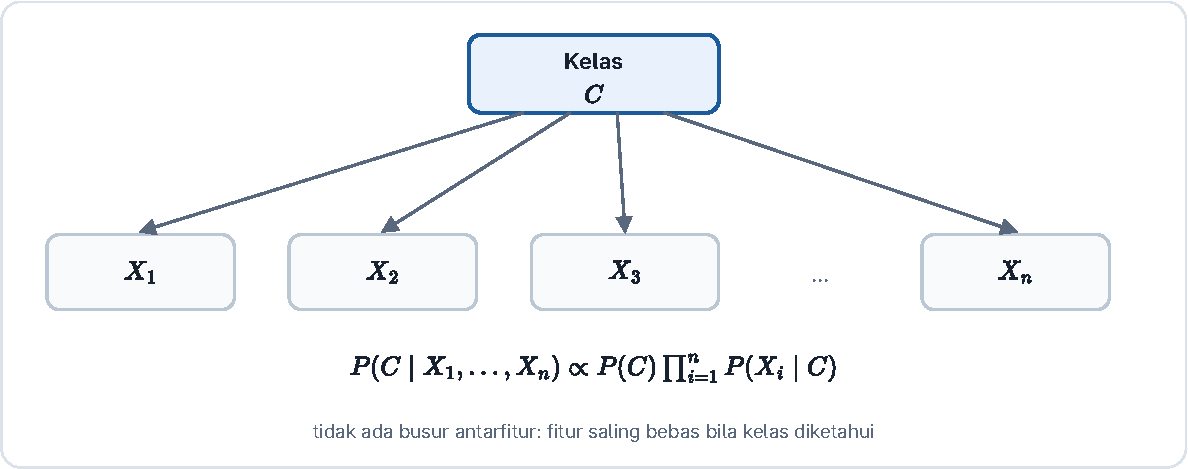
\includegraphics[width=0.78\textwidth]{diagram/naive_bayes.pdf}
    \caption{Struktur \textit{Naive Bayes} sebagai \textit{Bayesian network}.}
    \label{fig:teori-nb}
\end{figure}

\subsection{Validasi Model dan Metrik Evaluasi}
\textit{Train-test split} membagi data berlabel menjadi bagian latih dan validasi. Pembagian berstrata (\textit{stratified}) menjaga proporsi kelas tetap sama pada kedua bagian, yang penting ketika kelas tidak seimbang. \textit{k-fold cross-validation} membagi data menjadi $k$ lipatan. Setiap lipatan bergiliran menjadi validasi sementara $k-1$ lipatan lainnya menjadi data latih, lalu skor dirata-rata. Estimasi ini lebih stabil daripada satu pembagian, dengan syarat seluruh tahap persiapan data di-\textit{fit} ulang di dalam setiap lipatan. Skemanya ditunjukkan Gambar~\ref{fig:teori-kfold}.

\begin{figure}[htbp]
    \centering
    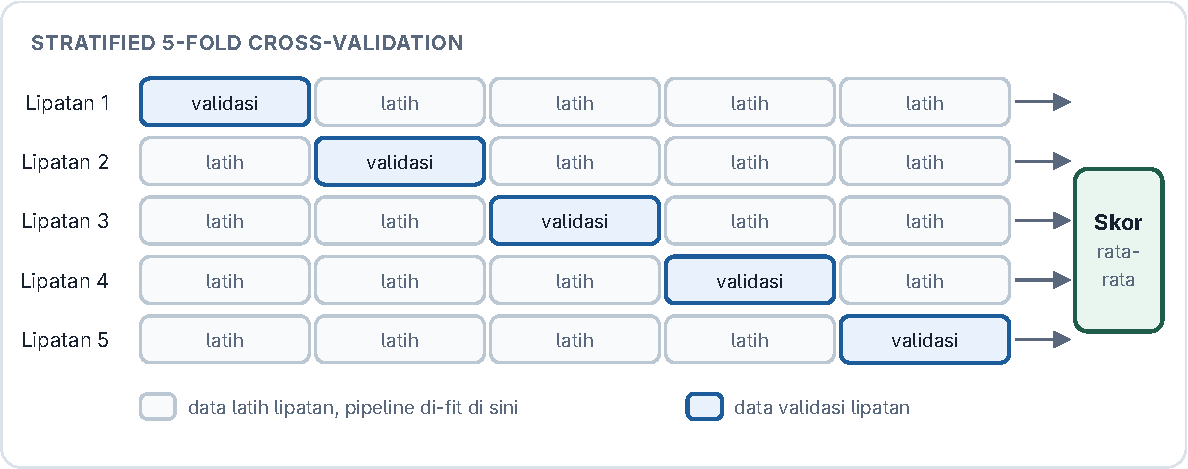
\includegraphics[width=0.8\textwidth]{diagram/kfold.pdf}
    \caption{\textit{Stratified 5-fold cross-validation}.}
    \label{fig:teori-kfold}
\end{figure}

Hasil klasifikasi biner dirangkum dalam \textit{confusion matrix} yang memuat \textit{true positive} (TP), \textit{true negative} (TN), \textit{false positive} (FP), dan \textit{false negative} (FN). Metrik yang digunakan adalah
\begin{equation}
    \mathrm{Acc}=\frac{TP+TN}{TP+TN+FP+FN},\quad
    \mathrm{Prec}=\frac{TP}{TP+FP},\quad
    \mathrm{Rec}=\frac{TP}{TP+FN},\quad
    F_1=\frac{2\,\mathrm{Prec}\cdot\mathrm{Rec}}{\mathrm{Prec}+\mathrm{Rec}}.
    \label{eq:metrics}
\end{equation}
Akurasi mudah ditafsirkan, tetapi pada data tidak seimbang model yang selalu menebak kelas mayoritas pun dapat memperoleh akurasi cukup tinggi. Presisi menjawab berapa bagian prediksi batal yang benar, sedangkan \textit{recall} menjawab berapa bagian pembatalan yang terdeteksi. ROC-AUC adalah luas di bawah kurva \textit{true positive rate} terhadap \textit{false positive rate} untuk seluruh ambang. Nilainya sama dengan peluang model memberi skor lebih tinggi kepada sampel positif acak daripada sampel negatif acak, sehingga dapat dihitung melalui statistik peringkat Mann--Whitney tanpa menetapkan ambang.

\subsection{\textit{Cost-Sensitive Classification}}\label{sec:teori-cost}
Pada banyak persoalan, jenis kesalahan berbeda memiliki biaya berbeda. Misalkan biaya FP adalah $c_{FP}$ dan biaya FN adalah $c_{FN}$. Untuk sampel dengan peluang positif $p$, memprediksi positif memberi biaya harapan $(1-p)\,c_{FP}$, sedangkan memprediksi negatif memberi $p\,c_{FN}$. Prediksi positif lebih murah bila $(1-p)c_{FP}<p\,c_{FN}$, sehingga ambang keputusan optimum adalah
\begin{equation}
    \tau^*=\frac{c_{FP}}{c_{FP}+c_{FN}}.
    \label{eq:cost-threshold}
\end{equation}
Dengan $c_{FP}=2$ dan $c_{FN}=1$, diperoleh $\tau^*=2/3$. Aturan ini hanya tepat jika peluang model terkalibrasi. Bila tidak, ambang dapat dicari secara empiris dengan meminimalkan biaya total $2\,FP+FN$ pada data validasi.
 Gambar~\ref{fig:teori-confusion} menunjukkan letak biaya pada \textit{confusion matrix}.

\begin{figure}[htbp]
    \centering
    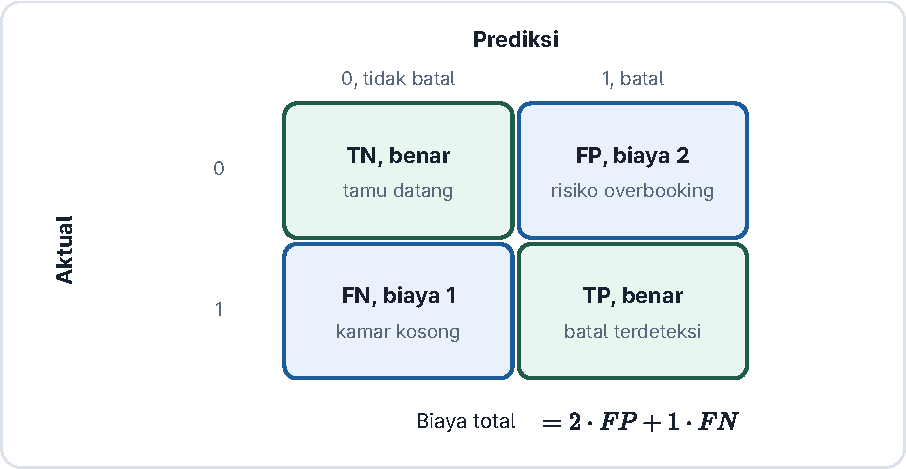
\includegraphics[width=0.6\textwidth]{diagram/confusion.pdf}
    \caption{\textit{Confusion matrix} dan biaya kesalahan pada persoalan pembatalan pemesanan.}
    \label{fig:teori-confusion}
\end{figure}

\subsection{Algoritma Optimasi Model}
Bagian ini merangkum algoritma optimasi di luar materi kelas yang dipakai untuk meningkatkan kinerja model.
\begin{enumerate}
    \setlength{\itemsep}{0pt}
    \item \textbf{FISTA}\\
    \textit{Gradient descent} proksimal (ISTA) memiliki laju konvergensi objektif $O(1/k)$. FISTA menambahkan momentum Nesterov. Langkah gradien dan \textit{soft-threshold} dihitung pada titik ekstrapolasi $\mathbf{z}_k=\boldsymbol{\theta}_k+\frac{t_k-1}{t_{k+1}}(\boldsymbol{\theta}_k-\boldsymbol{\theta}_{k-1})$ dengan $t_{k+1}=\bigl(1+\sqrt{1+4t_k^2}\bigr)/2$, sehingga laju konvergensinya menjadi $O(1/k^2)$. Ukuran langkah $1/L$ diturunkan dari konstanta Lipschitz gradien \textit{log-loss}, yaitu $L=\lambda_{\max}(\mathbf{X}^\top\mathbf{X}/n)/4$ ditambah koefisien L2. Karena tetap memakai operator proksimal, FISTA berlaku untuk L1 dan Elastic Net.
    \item \textbf{Adam}\\
    Adam menyimpan rata-rata bergerak gradien $m_t=\beta_1 m_{t-1}+(1-\beta_1)g_t$ dan kuadrat gradien $v_t=\beta_2 v_{t-1}+(1-\beta_2)g_t^2$. Setelah koreksi bias $\hat{m}_t=m_t/(1-\beta_1^t)$ dan $\hat{v}_t=v_t/(1-\beta_2^t)$, parameter diperbarui dengan $\theta\leftarrow\theta-\eta\,\hat{m}_t/(\sqrt{\hat{v}_t}+\epsilon)$. Setiap parameter memperoleh ukuran langkah sendiri, sehingga parameter dengan gradien kecil tetap bergerak cukup jauh. Adam dirancang untuk fungsi tujuan yang mulus, sehingga pada implementasi kelompok Adam hanya dipakai untuk penalti L2 atau tanpa penalti.
    \item \textbf{\textit{Cost-complexity pruning}}\\
    Pohon penuh dipangkas dengan meminimalkan Persamaan~\ref{eq:ccp}. Nilai $\alpha$ yang lebih besar menghasilkan pohon yang lebih kecil, dan $\alpha$ terbaik dipilih dengan validasi silang.
    \item \textbf{\textit{Random search}}\\
    Konfigurasi \textit{hyperparameter} diambil secara acak dari ruang pencarian dan dinilai dengan validasi silang. Pada ruang berdimensi tinggi yang hanya sebagian dimensinya berpengaruh, \textit{random search} lebih efisien daripada \textit{grid search} dengan anggaran percobaan yang sama.
    \item \textbf{Penalti MDL untuk atribut kontinu}\\
    Atribut kontinu dengan $N$ nilai berbeda memiliki $N-1$ kandidat ambang, sehingga peluang menemukan ambang yang tampak baik secara kebetulan meningkat. Quinlan mengusulkan pengurangan \textit{information gain} sebesar $\log_2(N-1)/|D|$, dengan $|D|$ jumlah sampel pada simpul. Penalti ini mengikuti prinsip \textit{minimum description length} (MDL), yaitu biaya untuk menyandikan pilihan ambang, dan atribut yang \textit{gain}-nya tidak positif setelah dikurangi penalti tidak dipakai.
    \item \textbf{Diskretisasi MDL pada \textit{Naive Bayes}}\\
    Interval kuantil diganti dengan ambang Fayyad--Irani pada Persamaan~\ref{eq:fayyad}. Ambang ditentukan oleh hubungan fitur dengan label, sehingga fitur yang jarang bernilai positif tetap dapat memiliki potongan.
    \item \textbf{Seleksi \textit{working set} orde kedua pada SMO}\\
    Indeks kedua pada SMO dipilih dengan kriteria $-b_{ij}^2/a_{ij}$ dari Fan, Chen, dan Lin. Kriteria berhenti tetap celah KKT pasangan pelanggar maksimal, sehingga solusi yang dicapai sama dan yang berubah hanya jumlah iterasi.
\end{enumerate}

\clearpage
\section{Pembahasan dan Implementasi}
\subsection{Struktur Repositori dan Antarmuka Model}
Repositori \texttt{IF3170\_G02\_nutellabear} memisahkan kode kelas dari notebook pengumpulan. Kelas model dan modul pendukung berada di \path{src/}, lalu di-\textit{import} atau disalin ke notebook templat asisten agar notebook dapat dijalankan pula di Kaggle. Hasil \textit{run} disimpan di \path{output/}, laporan di \path{docs/}, dan pengujian unit di \path{tests/}.

\begin{lstlisting}[language={},caption={Struktur repositori},label={lst:struktur}]
.
|-- T2-IF3170-2026-2027/   train.csv, test.csv, sample_submission.csv
|-- nb/                    notebook templat pengumpulan
|-- src/
|   |-- preprocessing.py   split, cleaning, langkah persiapan, pipeline
|   |-- evaluation.py      metrik, ROC-AUC, stratified k-fold, cross_validate
|   |-- knn.py, decision_tree.py, logreg.py, svm.py, naive_bayes.py
|   |-- knn_tuning.py, dtl_tuning.py     eksperimen optimasi model
|   |-- cost_sensitive.py, nb_graph.py, nb_compare.py, eda.py
|   |-- submission.py      make_submission, check_reproducible
|-- tests/                 pengujian unit per modul (pytest)
|-- output/                gambar, video, dan CSV submission
|-- docs/                  laporan
\end{lstlisting}

Kelima model memakai antarmuka yang seragam: \texttt{fit(X, y)}, \texttt{predict\_proba(X)} yang mengembalikan peluang kelas 1 berbentuk $(m,)$, \texttt{predict(X, threshold=0.5)}, \texttt{save(path)}, dan \texttt{load(path)}. Dengan antarmuka ini, modul evaluasi, validasi silang, \textit{cost-sensitive}, dan \textit{submission} dapat memanggil setiap model dengan cara yang sama. Implementasi \textit{from scratch} hanya memakai NumPy untuk perhitungan. Pustaka \textit{scikit-learn} dipakai untuk pembagian data, \textit{mutual information}, PCA, dan model pembanding.

\begin{figure}[htbp]
    \centering
    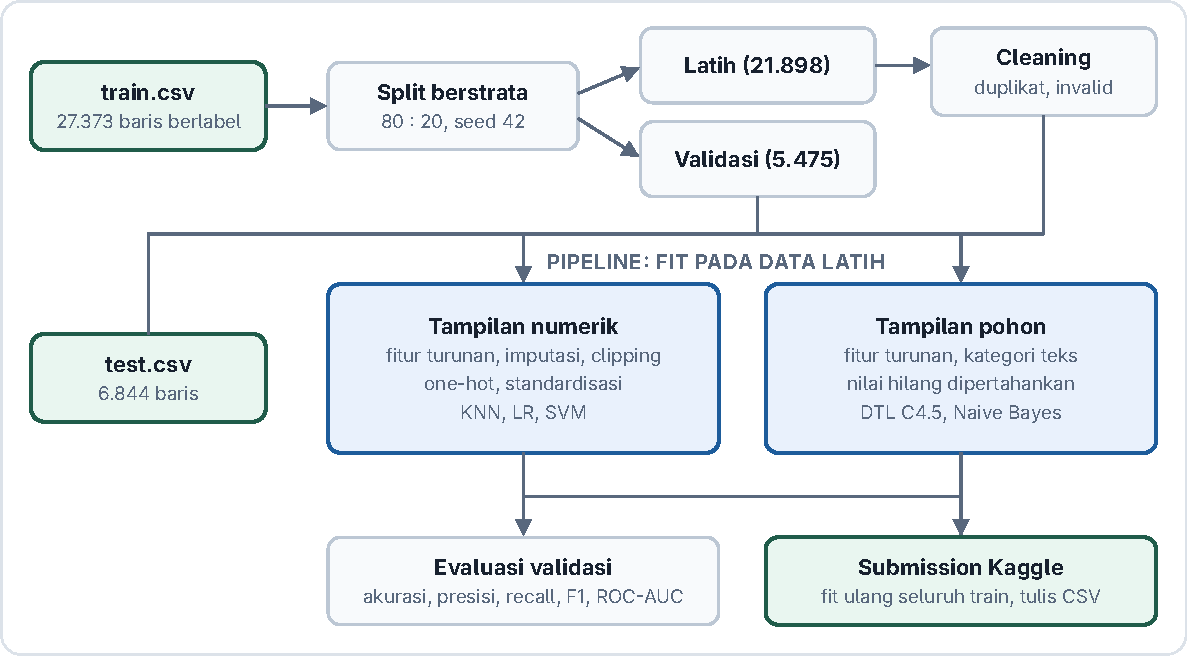
\includegraphics[width=\textwidth]{diagram/pipeline.pdf}
    \caption{Alur pengolahan data dari pembagian hingga evaluasi dan \textit{submission}.}
    \label{fig:pipeline}
\end{figure}

\subsection{\textit{Data Cleaning} dan \textit{Preprocessing}}\label{sec:preprocessing}
Gambar~\ref{fig:pipeline} merangkum alur pengolahan data. Seluruh langkah yang mempelajari statistik dari data dibungkus dalam kelas dengan metode \texttt{fit} dan \texttt{transform}, lalu dirangkai oleh \texttt{PreparationPipeline}. Pipeline di-\textit{fit} hanya pada data latih, sedangkan data validasi dan uji hanya di-\textit{transform}, sehingga tidak terjadi \textit{data leakage}.

\begin{lstlisting}[emph={PreparationPipeline,numeric_pipeline,tree_pipeline},caption={Pipeline dan dua tampilan data (\texttt{src/preprocessing.py})},label={lst:pipeline}]
class PreparationPipeline:
    def _run(self, df, fit):
        df = df.drop(columns=[ID_COL], errors="ignore")
        for step in self.steps:
            if callable(step):  # fungsi tanpa state, mis. construct_features
                df = step(df)
            else:
                df = (step.fit(df) if fit else step).transform(df)
        return df

def numeric_pipeline(select_k=None, pca=None):
    """Tampilan numerik (KNN, LR, SVM): tanpa NaN, one-hot, terskala."""
    steps = [construct_features, Imputer(), Clipper(), CategoricalEncoder(), Scaler()]
    ...

def tree_pipeline(impute=False):
    """Tampilan pohon (DTL, NB): kategori tetap teks, NaN dibiarkan."""
    return PreparationPipeline([construct_features] + ([Imputer()] if impute else []))
\end{lstlisting}

\subsubsection{Pembagian Data}
\texttt{split\_train\_val} membagi \path{train.csv} menjadi 80\% data latih (21.898 baris) dan 20\% data validasi (5.475 baris) secara berstrata terhadap \texttt{is\_canceled} dengan \texttt{seed=42}. Proporsi kelas batal pada kedua bagian sama, yaitu 32,77\%. Seluruh anggota memakai pembagian dan \textit{seed} yang sama agar angka antarmodel dapat dibandingkan. Validasi silang lima lipatan memakai fungsi \texttt{stratified\_kfold} buatan sendiri dengan \textit{seed} yang sama.

\subsubsection{Duplikat dan Data Tidak Valid}
\texttt{drop\_duplicates\_and\_invalid} hanya diterapkan pada data latih. Kelompok baris dengan fitur identik tetapi label berbeda dibuang seluruhnya, karena tidak ada cara menentukan label yang benar dan keberadaannya hanya menambah derau. Kelompok duplikat lain disisakan satu baris agar pola yang sama tidak berbobot ganda. Baris dengan nilai negatif atau tanpa tamu sama sekali dianggap mustahil dan dibuang. Pada data latih hasil pembagian, langkah ini membuang 2 baris berlabel konflik dan 40 duplikat, sehingga tersisa 21.856 baris.

Beberapa nilai yang tampak janggal sengaja dipertahankan karena mengandung informasi tentang pembatalan. Tabel~\ref{tab:nilai-janggal} menunjukkan bahwa pemesanan tanpa malam menginap dan pemesanan bertarif nol hampir tidak pernah batal. Kemungkinan besar keduanya mewakili pemesanan khusus, seperti \textit{day use} atau kamar gratis, sehingga membuangnya justru menghapus pola yang berguna. Data validasi dan uji tidak dibersihkan karena setiap barisnya tetap harus memperoleh prediksi.

\begin{table}[htbp]
    \centering
    \small
    \begin{tabular}{@{}l r r@{}}
        \toprule
        Kondisi pada data latih & Jumlah baris & Rasio batal \\
        \midrule
        Tanpa malam menginap & 49 & 0,0408 \\
        Tanpa tamu dewasa & 84 & 0,2976 \\
        Tarif per malam nol & 324 & 0,0062 \\
        Tanpa tamu sama sekali / nilai negatif & 0 & -- \\
        \bottomrule
    \end{tabular}
    \caption{Nilai janggal pada data latih beserta rasio pembatalannya.}
    \label{tab:nilai-janggal}
\end{table}

\subsubsection{Nilai Hilang}
Tampilan numerik mengisi nilai hilang dengan median untuk fitur numerik dan modus untuk fitur kategorikal. Median dipilih karena beberapa fitur, seperti tarif dan \texttt{days\_before\_arrival}, memiliki distribusi miring dengan pencilan. Nilai pengisi yang dipelajari dari data latih antara lain 57 hari untuk \texttt{days\_before\_arrival}, Rp1.647.000 untuk \texttt{nightly\_rate\_idr}, Breakfast untuk \texttt{meal\_package}, dan Type B untuk \texttt{room\_category}.

Untuk \texttt{special\_requests}, \texttt{Imputer} juga menambahkan kolom indikator \texttt{special\_requests\_missing}. Alasannya, rasio batal baris yang nilai ini hilang mencapai 0,4074, jauh di atas 0,3196 pada baris yang nilainya ada. Pola hilangnya data ini sendiri informatif, sehingga indikator mempertahankan informasi yang akan hilang bila nilai hanya diisi median. Fitur lain tidak menunjukkan perbedaan sebesar itu.

Tampilan pohon tidak mengimputasi nilai hilang. DTL C4.5 menangani nilai hilang dengan bobot pecahan, sedangkan \textit{Naive Bayes} cukup melewati fitur yang hilang ketika menghitung \textit{likelihood}. Dengan cara ini kedua model tidak bergantung pada nilai tebakan.

\subsubsection{Pencilan}
\texttt{Clipper} memotong \texttt{days\_before\_arrival}, \texttt{nightly\_rate\_idr}, dan \texttt{nightly\_rate\_per\_guest} ke persentil 1\% dan 99\% data latih. Ketiga fitur tersebut kontinu dan memiliki ekor panjang, sehingga nilai ekstremnya dapat mendominasi jarak KNN, kernel SVM, dan gradien \textit{logistic regression}. Batas atas yang dipelajari adalah 342 hari dan Rp3.408.000, dan sekitar 218 baris latih terpotong pada setiap fitur. Fitur hitungan seperti \texttt{prior\_cancellations} tidak dipotong karena persentil 99\%-nya bernilai 0. Pemotongan akan menghapus informasi penting karena 183 baris dengan \texttt{prior\_cancellations} positif hanya memiliki rasio batal 0,044, jauh di bawah 0,330 pada baris lain.

\subsubsection{Konstruksi Fitur}
\texttt{construct\_features} menambahkan tiga fitur turunan: \texttt{total\_nights} (jumlah malam akhir pekan dan hari kerja), \texttt{total\_guests} (jumlah tamu dewasa dan anak), serta \texttt{nightly\_rate\_per\_guest} (tarif dibagi jumlah tamu). Fitur-fitur ini merangkum besar pemesanan dan harga per orang, yang secara intuitif berkaitan dengan komitmen tamu. Korelasi Spearman ketiganya terhadap target berturut-turut 0,089, 0,081, dan 0,035, sehingga hubungannya dengan target ada tetapi lemah. Fitur turunan dipakai pada tampilan numerik dan tampilan pohon. Konfigurasi \textit{Naive Bayes} memakai fitur asli karena validasi silang menunjukkan fitur turunan menurunkan akurasinya (Subbab~\ref{sec:hasil-nb}).

\subsubsection{\textit{Encoding} dan Penskalaan}
\texttt{CategoricalEncoder} melakukan \textit{one-hot encoding} dengan daftar kategori dari data latih: 4 kategori \texttt{meal\_package}, 7 kategori \texttt{room\_category}, dan 5 kategori \texttt{booking\_channel}. Kategori yang tidak dikenal pada data baru dikodekan sebagai vektor nol sehingga tidak menimbulkan galat. \textit{One-hot} dipilih karena ketiga fitur bersifat nominal. Pengodean ordinal akan memaksakan urutan yang sebenarnya tidak ada sehingga memengaruhi jarak serta bobot linear.

\texttt{Scaler} melakukan standardisasi dengan rata-rata dan simpangan baku data latih. Kolom konstan diberi skala 1 untuk menghindari pembagian dengan nol. Setelah transformasi, rata-rata fitur pada data validasi mendekati 0 dan simpangan bakunya mendekati 1. Hasil akhir tampilan numerik adalah 34 kolom tanpa nilai hilang. Tampilan pohon berisi 20 kolom dengan kategori asli dan 17.990 sel bernilai hilang pada data latih.

\subsubsection{Seleksi Fitur, Reduksi Dimensi, dan Ketidakseimbangan Kelas}
Ketiga teknik ini diimplementasikan sebagai langkah opsional dan diuji pada KNN, karena KNN paling peka terhadap fitur yang tidak relevan dan dimensi tinggi. \texttt{FeatureSelector} memilih $k$ fitur dengan \textit{mutual information} tertinggi terhadap target. Fitur paling informatif adalah \texttt{days\_before\_arrival} (0,1020), \texttt{special\_requests} (0,0376), dan \texttt{nightly\_rate\_idr} (0,0268). \texttt{DimReducer} menerapkan PCA dan membutuhkan 25 dari 34 komponen untuk melampaui 95\% ragam kumulatif. Karena ragam tersebar pada banyak komponen, PCA tidak banyak memampatkan data ini. \texttt{handle\_imbalance} melakukan \textit{random oversampling} kelas minoritas dari 7.161 menjadi 14.695 baris, hanya pada data latih. Hasil ketiga variasi dibahas pada Subbab~\ref{sec:hasil-knn}. Pipeline baku tidak memakainya.

\subsection{Implementasi \textit{k-Nearest Neighbors}}
Kelas \texttt{KNN} pada \path{src/knn.py} menyimpan salinan data latih pada \texttt{fit}. Matriks jarak dihitung secara tervektorisasi per \textit{batch} 256 baris kueri agar memori tetap aman. Matriks penuh $5.475\times21.856$ bertipe \textit{float64} akan memerlukan sekitar 1 GB. Untuk jarak Euclidean, identitas $\|\mathbf{a}-\mathbf{b}\|^2=\|\mathbf{a}\|^2+\|\mathbf{b}\|^2-2\mathbf{a}^\top\mathbf{b}$ memungkinkan perhitungan dengan satu perkalian matriks. Untuk orde Minkowski lain, selisih diakumulasi per fitur agar tidak terbentuk larik tiga dimensi.

\begin{lstlisting}[emph={_pairwise_distances,kneighbors},caption={Perhitungan jarak dan pencarian tetangga (\texttt{src/knn.py})},label={lst:knn}]
def _pairwise_distances(self, Xq):
    p = {"euclidean": 2, "manhattan": 1}.get(self.metric, self.p)
    if p == 2:  # ||a-b||^2 = ||a||^2 + ||b||^2 - 2ab
        sq = (Xq ** 2).sum(1)[:, None] + (self.X_ ** 2).sum(1)[None, :] - 2 * Xq @ self.X_.T
        return np.sqrt(np.maximum(sq, 0))
    D = np.zeros((len(Xq), len(self.X_)))
    for j in range(Xq.shape[1]):  # per fitur, hindari array 3D
        D += np.abs(Xq[:, j, None] - self.X_[None, :, j]) ** p
    return D if p == 1 else D ** (1 / p)

def kneighbors(self, X):
    for s in range(0, len(X), self.batch_size):
        D = self._pairwise_distances(X[s:s + self.batch_size])
        nn = np.argpartition(D, self.k - 1, axis=1)[:, :self.k]  # k terkecil
        ...
\end{lstlisting}

Pemilihan $k$ tetangga memakai \texttt{np.argpartition} yang berjalan dalam waktu linear, lalu hanya $k$ jarak terpilih yang diurutkan. \texttt{predict\_proba} mengikuti Persamaan~\ref{eq:knn-proba}. Pada pembobotan \textit{distance}, bila ada tetangga berjarak nol, hanya titik identik tersebut yang dihitung, sesuai perilaku \textit{scikit-learn}.

\subsection{Implementasi \textit{Decision Tree Learning} (C4.5)}
Kelompok memilih C4.5 karena varian ini secara alami menangani atribut numerik, atribut kategorikal, dan nilai hilang, sesuai kebutuhan dataset ini. Kelas \texttt{DecisionTree} pada \path{src/decision_tree.py} menyimpan simpul sebagai \texttt{TreeNode} berisi jumlah kelas berbobot, fitur pemisah, ambang atau kategori, anak, dan peluang cabang untuk nilai hilang.

Untuk atribut numerik, \texttt{\_best\_numeric} mengurutkan nilai yang diketahui, lalu menghitung jumlah kelas kumulatif sehingga seluruh kandidat ambang dievaluasi sekaligus dalam $O(n\log n)$. \textit{Gain} pada sampel diketahui dikalikan proporsi bobot yang diketahui, dan nilai hilang diperlakukan sebagai partisi tambahan pada \textit{split information}, sesuai Subbab dasar teori.

\begin{lstlisting}[emph={_best_numeric},caption={Evaluasi seluruh ambang numerik secara kumulatif (\texttt{src/decision\_tree.py}, diringkas)},label={lst:dtl-numeric}]
positions = np.flatnonzero(values[:-1] < values[1:])  # batas antar nilai berbeda
cumulative, positive = np.cumsum(w), np.cumsum(w * labels)
left_w, left_pos = cumulative[positions], positive[positions]
right_w, right_pos = cumulative[-1] - left_w, positive[-1] - left_pos
known_w, missing_w = cumulative[-1], weights[~known].sum()
gain = np.maximum(0.0, known_w / (known_w + missing_w) *
                  (parent_h - (left_w * _entropy_counts(left)
                               + right_w * _entropy_counts(right)) / known_w))
split_info = _entropy_counts(np.column_stack((masses, np.full(len(masses), missing_w))))
ratios = np.divide(gain, split_info, out=np.zeros_like(gain), where=split_info > 1e-12)
\end{lstlisting}

Atribut kategorikal dipecah per kategori (\textit{multiway}) dan tidak diuji ulang pada keturunannya. Pemilihan atribut mengikuti aturan C4.5: hanya kandidat dengan \textit{gain} minimal sebesar rata-rata yang dibandingkan \textit{gain ratio}-nya.

\begin{lstlisting}[caption={Pemilihan split dan pembagian bobot pecahan (\texttt{src/decision\_tree.py}, diringkas)},label={lst:dtl-split}]
average_gain = np.mean([s.gain for s in candidates])
eligible = [s for s in candidates if s.gain >= average_gain - 1e-12]
split = max(eligible, key=lambda s: s.ratio)
...
for branch, key in enumerate(keys):
    probability = float(split.probabilities[branch])
    mask = (branches == branch) | missing          # sampel hilang ikut ke semua cabang
    child_w = w[mask] * np.where(missing[mask], probability, 1.0)
\end{lstlisting}

Pohon dibangun secara iteratif dengan \textit{stack}, bukan rekursi, sehingga tidak ada risiko melampaui batas rekursi Python pada data besar. Pertumbuhan berhenti apabila simpul murni, jumlah sampel kurang dari \texttt{min\_samples\_split}, kedalaman mencapai \texttt{max\_depth} (baku 20), atau tidak ada kandidat dengan \textit{gain} melebihi \texttt{min\_gain}. Pada prediksi, sampel dengan nilai hilang atau kategori baru menelusuri seluruh cabang, dan peluang daun digabung menurut bobot cabang.

\subsection{Implementasi \textit{Logistic Regression}}
Kelas \texttt{LogisticRegression} pada \path{src/logreg.py} meminimalkan rata-rata \textit{log-loss} ditambah penalti (Persamaan~\ref{eq:logloss} dan~\ref{eq:reg}). Fungsi sigmoid ditulis stabil secara numerik dengan memisahkan kasus $z\geq0$ dan $z<0$, sehingga tidak terjadi \textit{overflow} untuk $|z|$ besar. Regularisasi dirancang sebagai hierarki kelas \texttt{Regularizer} dengan subkelas \texttt{L1}, \texttt{L2}, dan \texttt{ElasticNet}. Setiap subkelas menyediakan gradien bagian mulus (\texttt{grad\_smooth}) dan operator proksimal bagian L1 (\texttt{prox}).

\begin{lstlisting}[emph={ElasticNet,_soft_threshold},caption={Regularizer Elastic Net dengan langkah proksimal (\texttt{src/logreg.py})},label={lst:lr-reg}]
def _soft_threshold(w, t):
    return np.sign(w) * np.maximum(np.abs(w) - t, 0.0)

class ElasticNet(Regularizer):
    def grad_smooth(self, w):
        return self.alpha * (1 - self.l1_ratio) * w
    def prox(self, w, step):
        return _soft_threshold(w, step * self.alpha * self.l1_ratio)
\end{lstlisting}

Setiap iterasi melakukan langkah gradien pada \textit{log-loss} dan bagian L2, lalu menerapkan \textit{soft-threshold} untuk bagian L1. Dengan cara ini, bobot fitur yang tidak berguna menjadi tepat nol, bukan hanya mendekati nol. Bias tidak diregularisasi. Pelatihan berhenti apabila perubahan objektif antar-\textit{epoch} lebih kecil dari \texttt{tol}, dan riwayat objektif serta parameter disimpan pada \texttt{history\_} untuk keperluan video lintasan parameter.

\begin{lstlisting}[caption={Langkah pembaruan \textit{gradient descent} proksimal (\texttt{src/logreg.py}, diringkas)},label={lst:lr-fit}]
err = sigmoid(X[idx] @ w + b) - y[idx]
grad_w = X[idx].T @ err / len(idx) + reg.grad_smooth(w)
grad_b = err.mean()
w = reg.prox(w - self.lr * grad_w, self.lr)   # soft-threshold untuk bagian L1
b -= self.lr * grad_b
\end{lstlisting}

Optimizer tambahan ditempatkan pada subkelas \texttt{OptimizedLogisticRegression} di \path{src/logreg_optim.py} agar kelas induk tidak berubah. Subkelas ini menyediakan \texttt{optimizer="fista"} dan \texttt{optimizer="adam"}. Pada FISTA, laju belajar baku adalah $1/L$, dengan $\lambda_{\max}$ dihitung melalui iterasi pangkat pada matriks data yang diberi kolom satu untuk bias.

\begin{lstlisting}[caption={Satu iterasi FISTA (\texttt{src/logreg\_optim.py}, diringkas)},label={lst:fista}]
t_next = (1 + np.sqrt(1 + 4 * momentum_t ** 2)) / 2
z = theta + (momentum_t - 1) / t_next * (theta - previous)   # titik ekstrapolasi
g = gradient(z, np.arange(n))
new = z - self.lr * g
new[1:] = reg.prox(new[1:], self.lr)                          # bias tidak diregularisasi
previous, theta, momentum_t = theta, new, t_next
\end{lstlisting}

Konfigurasi baku memakai \textit{batch} penuh, laju belajar 0,1, $\alpha=0{,}01$, dan \texttt{l1\_ratio}=0,5. Hubungan dengan \textit{scikit-learn} adalah $\alpha=1/(C\,n)$, karena \textit{scikit-learn} meminimalkan $C\sum_i\ell_i+R(\mathbf{w})$. Hubungan ini dipakai agar kedua implementasi membandingkan fungsi tujuan yang sama.

\subsection{Implementasi \textit{Support Vector Machine}}
Kelas \texttt{SVM} pada \path{src/svm.py} menyelesaikan bentuk dual (Persamaan~\ref{eq:svm-dual}) dengan SMO. Setiap kernel adalah kelas dengan metode \texttt{compute(A, B)} yang mengembalikan matriks kernel secara tervektorisasi. Nilai baku $\gamma$ untuk kernel polinomial dan Gaussian adalah $1/m$ dengan $m$ jumlah fitur, sesuai opsi \texttt{gamma='auto'} pada \textit{scikit-learn}.

\begin{lstlisting}[emph={_smo},caption={Iterasi SMO dengan pemilihan \textit{maximal violating pair} (\texttt{src/svm.py})},label={lst:smo}]
for it in range(self.max_iter):
    up  = ((y > 0) & (alpha < C)) | ((y < 0) & (alpha > 0))
    low = ((y > 0) & (alpha > 0)) | ((y < 0) & (alpha < C))
    score = -y * G
    i = np.flatnonzero(up)[np.argmax(score[up])]
    j = np.flatnonzero(low)[np.argmin(score[low])]
    gap = score[i] - score[j]
    if gap < self.tol:          # KKT terpenuhi dalam toleransi
        self.converged_ = True
        break
    eta = max(diagK[i] + diagK[j] - 2 * K[i, j], 1e-12)
    t = min(gap / eta,
            C - alpha[i] if y[i] > 0 else alpha[i],
            alpha[j] if y[j] > 0 else C - alpha[j])
    alpha[i] += y[i] * t
    alpha[j] -= y[j] * t
    G += y * t * (K[:, i] - K[:, j])
\end{lstlisting}

Vektor $G$ menyimpan gradien objektif dual dan diperbarui secara inkremental hanya dengan dua kolom matriks kernel, sehingga setiap iterasi berjalan dalam $O(n)$. Setelah konvergen, bias $b$ dihitung dari rata-rata \textit{support vector} bebas ($0<\alpha_i<C$), dan hanya sampel dengan $\alpha_i>10^{-8}$ yang disimpan sebagai \textit{support vector}.

Strategi skala data menjadi keputusan desain terpenting pada SVM. Matriks kernel penuh untuk 21.856 baris latih memerlukan sekitar 3,8 GB dalam presisi ganda. Karena itu, apabila jumlah data melebihi \texttt{max\_samples}, SVM dilatih pada subsampel berstrata (baku 4.000 baris) dengan matriks kernel penuh di-\textit{cache}. Hingga 5.000 baris di luar subsampel dipakai untuk \textit{Platt scaling}, sehingga kalibrasi peluang tidak dilakukan pada data yang sama dengan pelatihan SVM. Parameter Platt dicari dengan metode Newton dan target ter-\textit{smoothing} menurut Lin dkk.. Subkelas \texttt{SVMWSS2} pada \path{src/svm_wss.py} hanya mengganti pemilihan indeks $j$ pada SMO dengan kriteria orde kedua. Kandidat $j$ dibatasi pada $I_{\mathrm{low}}$ dengan skor lebih kecil daripada skor $i$, lalu dipilih yang meminimalkan $-b_{ij}^2/a_{ij}$, dengan $a_{ij}$ diganti $10^{-12}$ bila tidak positif. Kriteria berhenti dan perhitungan bias sama dengan kelas induk.

\subsection{Implementasi \textit{Naive Bayes}}
Kelas \texttt{NaiveBayes} pada \path{src/naive_bayes.py} menerima tampilan data dengan kategori asli. Fitur numerik dengan lebih dari sepuluh nilai unik didiskretisasi, sedangkan fitur lain diperlakukan sebagai kategori. Parameter \texttt{discretization} memilih cara diskretisasi. Nilai baku \texttt{"quantile"} memakai 20 interval kuantil, sedangkan \texttt{"mdl"} memakai ambang Fayyad--Irani yang dihitung dari label data latih dengan nilai hilang diabaikan. Setiap fitur memiliki satu tingkat tambahan untuk kategori yang tidak dikenal pada data latih, sehingga data baru tidak menimbulkan galat.

\begin{lstlisting}[emph={fit,predict_proba},caption={Estimasi \textit{likelihood} dengan Laplace smoothing dan normalisasi \textit{log-sum-exp} (\texttt{src/naive\_bayes.py}, diringkas)},label={lst:nb}]
n_class = np.bincount(y, minlength=2)
self.log_prior_ = np.log((n_class + self.alpha) / (len(y) + 2 * self.alpha))
for c in self.columns_:
    codes = self._codes(c, col)              # -1 untuk nilai hilang
    counts = np.zeros((2, n_levels + 1))
    for k in (0, 1):
        seen = codes[(y == k) & (codes >= 0)]
        counts[k] = np.bincount(seen, minlength=n_levels + 1)
    self.log_lik_[c] = np.log((counts + self.alpha) /
                              (counts.sum(1, keepdims=True) + self.alpha * (n_levels + 1)))

# predict_proba
score = np.tile(self.log_prior_, (len(X), 1))
for c in self.columns_:
    codes = self._codes(c, X[c]); known = codes >= 0
    score[known] += self.log_lik_[c][:, codes[known]].T   # fitur hilang dilewati
peak = score.max(axis=1, keepdims=True)
log_norm = peak + np.log(np.exp(score - peak).sum(axis=1, keepdims=True))
return np.exp(score - log_norm)[:, 1]
\end{lstlisting}

Perhitungan dilakukan dalam ruang log, dan fitur yang nilainya hilang tidak menyumbang \textit{likelihood}. Pendekatan ini setara dengan marginalisasi fitur tersebut, karena $\sum_v P(x_j=v\mid C)=1$. Normalisasi \textit{log-sum-exp} mencegah \textit{underflow}, dan jumlah peluang kedua kelas selalu satu.

\subsection{Evaluasi, Penyimpanan Model, dan \textit{Submission}}
Modul \path{src/evaluation.py} mengimplementasikan \textit{confusion matrix}, akurasi, presisi, \textit{recall}, F1, dan ROC-AUC. ROC-AUC dihitung sebagai statistik Mann--Whitney dengan rata-rata peringkat untuk skor kembar. Fungsi \texttt{cross\_validate} menerima fungsi \texttt{prepare(train\_df, val\_df)} yang dipanggil pada setiap lipatan, sehingga pipeline di-\textit{fit} ulang pada bagian latih lipatan tersebut.

Model disimpan dengan \texttt{pickle}, kecuali \texttt{WeightedKNN} yang memakai format \texttt{.npz} tanpa \textit{pickle}. Notebook menyimpan lima konfigurasi pengumpulan serta eksperimen SVM Gaussian 12.000 baris, memuat ulang masing-masing, lalu memastikan peluang hasil muat ulang cocok dalam toleransi $10^{-12}$ dan label prediksinya identik. Keenam pemeriksaan lolos.

Fungsi \texttt{make\_submission} membersihkan seluruh \path{train.csv}, melatih ulang pipeline dan model pada data tersebut, lalu hanya men-\textit{transform} \path{test.csv}. Keluarannya adalah CSV berisi \texttt{id} dan \texttt{is\_canceled} dengan 6.844 baris, sama dengan format \path{sample_submission.csv}. Fungsi \texttt{check\_reproducible} membandingkan dua berkas \textit{submission} tanpa memperhatikan urutan baris.

\clearpage
\section{Hasil Eksperimen dan Analisis}
\subsection{Rancangan Eksperimen}
Seluruh model dievaluasi pada 5.475 baris validasi yang sama, hasil pembagian berstrata dengan \texttt{seed=42}. Model dilatih pada 21.856 baris latih yang telah dibersihkan. Untuk konfigurasi terpilih, validasi silang lima lipatan dijalankan pada seluruh \path{train.csv}, dengan pipeline di-\textit{fit} ulang pada setiap lipatan. Metrik berbasis label memakai ambang 0,5, kecuali pada analisis \textit{cost-sensitive}.

Metrik utama pemilihan konfigurasi adalah akurasi, sesuai metrik yang diasumsikan untuk leaderboard Kaggle. F1 kelas batal dan ROC-AUC dilaporkan sebagai pelengkap, karena akurasi saja dapat menyamarkan kemampuan model mendeteksi kelas minoritas. Setiap akurasi dibandingkan dengan baseline kelas mayoritas sebesar 0,6723.

Angka pada bab ini berasal dari eksekusi ulang notebook pengumpulan dari sel pertama hingga terakhir dengan versi pustaka pada \path{requirements.txt}. Eksekusi ulang menghasilkan CSV KNN, DTL, \textit{logistic regression}, dan \textit{Naive Bayes} yang identik dengan berkas pada \path{output/}. CSV SVM polinomial berbeda pada 9 dari 6.844 baris, yang diduga berasal dari perbedaan pembulatan aritmetika titik mengambang pada SMO. Selisih kecil juga terlihat pada metrik DTL dibanding catatan di notebook (akurasi 0,8451 berbanding 0,8449), tetapi CSV DTL tetap identik.

\subsection{Hasil per Algoritma}
\subsubsection{\textit{k-Nearest Neighbors}}\label{sec:hasil-knn}
Tabel~\ref{tab:knn-grid} memperlihatkan pengaruh $k$ dan pembobotan pada jarak Euclidean. Pembobotan jarak selalu lebih baik daripada pembobotan seragam pada setiap $k$, dengan selisih akurasi 1,2 hingga 3,0 poin persentase. Pembobotan seragam mencapai akurasi tertinggi pada $k=5$ lalu menurun, sedangkan pembobotan jarak membaik hingga $k=15$ dan tetap stabil sesudahnya. Hal ini terjadi karena bobot $1/d$ meredam pengaruh tetangga jauh yang ikut terhitung ketika $k$ membesar.

\begin{table}[htbp]
    \centering
    \small
    \begin{tabular}{@{}r l r r r r r@{}}
        \toprule
        $k$ & Bobot & Akurasi & Presisi & \textit{Recall} & F1 & ROC-AUC \\
        \midrule
        5 & \textit{uniform} & 0,8188 & 0,7416 & 0,6862 & 0,7128 & 0,8743 \\
        5 & \textit{distance} & 0,8312 & 0,7544 & 0,7191 & 0,7363 & 0,8878 \\
        15 & \textit{uniform} & 0,8179 & 0,7589 & 0,6511 & 0,7009 & 0,8827 \\
        15 & \textit{distance} & \textbf{0,8429} & 0,7876 & 0,7129 & \textbf{0,7484} & 0,9047 \\
        25 & \textit{uniform} & 0,8126 & 0,7623 & 0,6221 & 0,6851 & 0,8779 \\
        25 & \textit{distance} & 0,8413 & 0,7937 & 0,6968 & 0,7421 & \textbf{0,9055} \\
        41 & \textit{uniform} & 0,8119 & 0,7656 & 0,6137 & 0,6813 & 0,8722 \\
        41 & \textit{distance} & 0,8413 & 0,8013 & 0,6856 & 0,7390 & 0,9049 \\
        \bottomrule
    \end{tabular}
    \caption{Pengaruh $k$ dan pembobotan pada KNN (jarak Euclidean, data validasi).}
    \label{tab:knn-grid}
\end{table}

Dengan $k=15$ dan pembobotan jarak, jarak Manhattan memberi akurasi 0,8489, lebih tinggi daripada Euclidean (0,8429) dan Minkowski $p=3$ (0,8378). Jarak Manhattan tidak mengkuadratkan selisih, sehingga satu fitur dengan selisih besar tidak mendominasi jarak. Sifat ini menguntungkan pada data campuran yang memuat banyak kolom \textit{one-hot}. Konfigurasi $k=15$, Manhattan, bobot jarak dipilih untuk \textit{submission}.

\begin{table}[htbp]
    \centering
    \small
    \begin{tabular}{@{}l r r r r r@{}}
        \toprule
        Variasi \textit{preprocessing} & Akurasi & Presisi & \textit{Recall} & F1 & ROC-AUC \\
        \midrule
        Pipeline baku & 0,8489 & 0,7998 & 0,7191 & 0,7573 & 0,9106 \\
        20 fitur \textit{mutual information} teratas & 0,8515 & 0,8056 & 0,7207 & 0,7608 & 0,9099 \\
        PCA 95\% ragam (25 komponen) & 0,8462 & 0,7920 & 0,7196 & 0,7541 & 0,9053 \\
        \textit{Random oversampling} & 0,8201 & 0,6820 & 0,8450 & 0,7548 & 0,9063 \\
        \bottomrule
    \end{tabular}
    \caption{Pengaruh seleksi fitur, PCA, dan \textit{oversampling} pada KNN terpilih.}
    \label{tab:knn-variasi}
\end{table}

Tabel~\ref{tab:knn-variasi} menunjukkan bahwa seleksi 20 fitur menaikkan akurasi sebesar 0,26 poin persentase, karena kolom yang hampir tidak informatif berhenti menambah derau pada jarak. Kenaikan tersebut kecil dan hanya teramati pada satu pembagian, sehingga pipeline baku tetap dipakai untuk menjaga \textit{submission} yang sudah ada tetap \textit{reproducible}. PCA sedikit menurunkan kinerja karena proyeksi linear mencampur fitur penting dengan fitur lemah. \textit{Oversampling} menaikkan \textit{recall} dari 0,7191 menjadi 0,8450, tetapi presisi dan akurasi turun tajam. Hasil ini wajar, karena salinan sampel minoritas memperbanyak tetangga positif di sekitar setiap titik kueri sehingga model lebih sering menebak batal.

Validasi silang lima lipatan untuk konfigurasi terpilih menghasilkan rata-rata akurasi 0,8429, F1 0,7484, dan ROC-AUC 0,9049. Akurasi per lipatan berkisar 0,8409 hingga 0,8453. Rentang yang sempit ini menunjukkan bahwa kinerja KNN stabil terhadap perubahan pembagian data, dan skor pada pembagian validasi utama (0,8489) sedikit di atas rata-rata.

\subsubsection{\textit{Decision Tree Learning}}
Pohon C4.5 tanpa pemangkasan tumbuh hingga 4.634 simpul dengan kedalaman maksimum 20. Pada data validasi, pohon ini memperoleh akurasi 0,8451, presisi 0,7877, \textit{recall} 0,7219, F1 0,7533, dan ROC-AUC 0,8980. Kinerjanya hampir setara dengan KNN terbaik, padahal pohon bekerja langsung pada kategori asli dan nilai hilang tanpa imputasi.

Gambar~\ref{fig:dtl-top3} menampilkan tiga simpul pemisah teratas. Akar memilih \texttt{days\_before\_arrival} dengan ambang 154,5 hari. Pada pemesanan yang lebih dekat dengan kedatangan, peluang batal turun menjadi 23,7\%, dan tamu dengan riwayat pemesanan selesai (\texttt{prior\_completed\_bookings} $>0{,}5$) hampir tidak pernah batal (0,4\%). Pada pemesanan lebih dari 154,5 hari, peluang batal naik menjadi 70,9\% dan mencapai 89,9\% untuk tarif di atas sekitar Rp1,69 juta. Struktur ini konsisten dengan temuan \textit{data understanding} bahwa \texttt{days\_before\_arrival} adalah fitur paling informatif.

\begin{figure}[htbp]
    \centering
    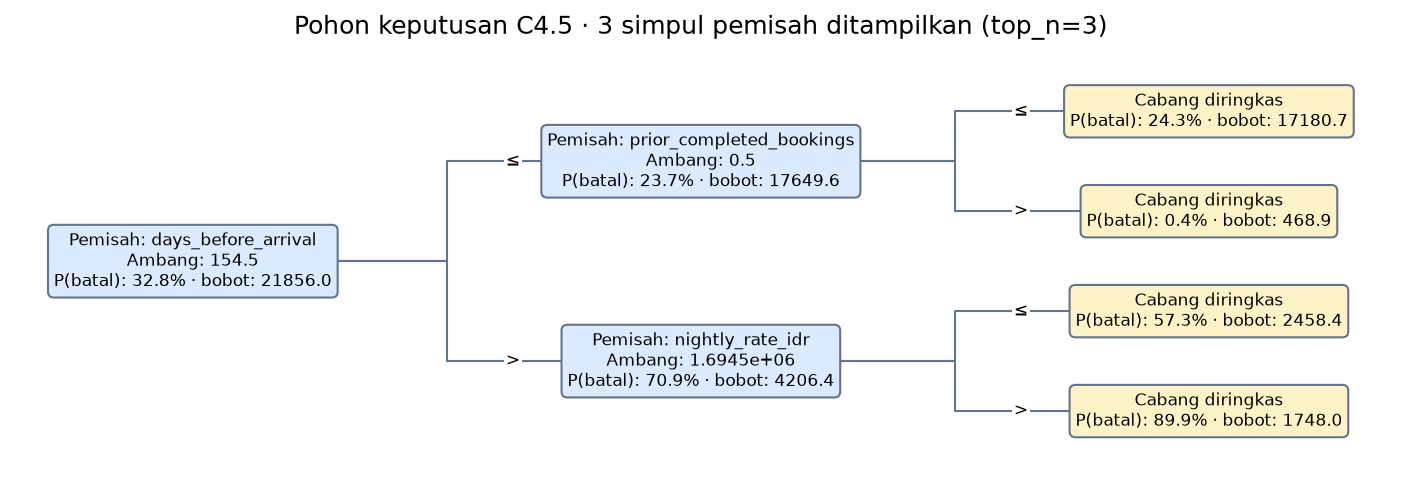
\includegraphics[width=\textwidth]{output/decision_tree_top_3.png}
    \caption{Visualisasi pohon C4.5 dengan \texttt{top\_n=3}. Simpul kuning masih memiliki keturunan yang diringkas.}
    \label{fig:dtl-top3}
\end{figure}

Parameter \texttt{top\_n} membatasi jumlah simpul pemisah yang dibuka secara melebar dari akar. Simpul yang masih memiliki anak setelah batas tercapai ditandai ``Cabang diringkas''. Gambar~\ref{fig:dtl-top7} menampilkan \texttt{top\_n=7} dengan aturan yang lebih rinci.

\begin{figure}[htbp]
    \centering
    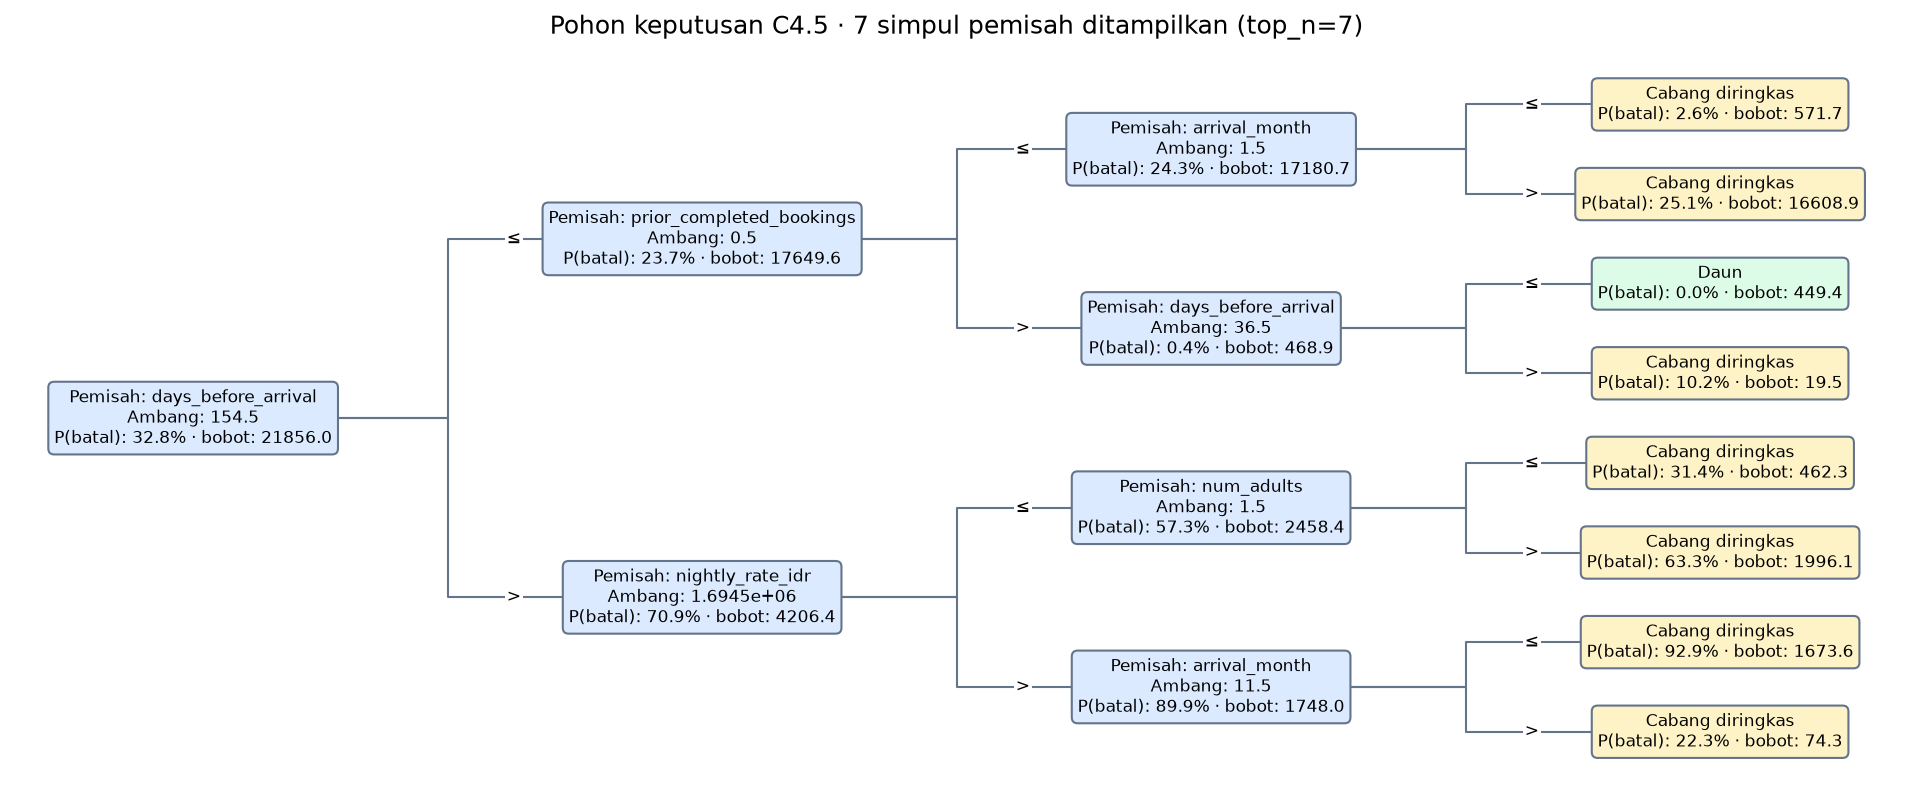
\includegraphics[width=\textwidth]{output/decision_tree_top_7.png}
    \caption{Visualisasi pohon C4.5 dengan \texttt{top\_n=7}.}
    \label{fig:dtl-top7}
\end{figure}

\subsubsection{\textit{Logistic Regression}}
Tabel~\ref{tab:lr} merangkum ketiga regularisasi dengan $\alpha=0{,}01$. Ketiganya konvergen dan menghasilkan akurasi yang sangat berdekatan, yaitu 0,7956 hingga 0,7980. Perbedaan utamanya terletak pada jumlah bobot yang bernilai nol. L1 menghasilkan 22 dari 34 bobot tepat nol, Elastic Net 19, dan L2 tidak ada. Hasil ini sesuai teori pada Gambar~\ref{fig:teori-lr}. Model L1 hanya memakai 12 fitur tetapi akurasinya turun kurang dari 0,25 poin persentase, sehingga sebagian besar fitur tidak menambah daya pisah linear. Elastic Net dipilih untuk \textit{submission} karena akurasinya tertinggi.

\begin{table}[htbp]
    \centering
    \small
    \begin{tabular}{@{}l r r r r r r r@{}}
        \toprule
        Penalti & \textit{Epoch} & Bobot nol & Akurasi & Presisi & \textit{Recall} & F1 & ROC-AUC \\
        \midrule
        L1 & 1.752 & 22 & 0,7956 & 0,7433 & 0,5747 & 0,6482 & 0,8507 \\
        L2 & 1.322 & 0 & 0,7965 & 0,7374 & 0,5886 & 0,6547 & 0,8538 \\
        Elastic Net & 1.142 & 19 & \textbf{0,7980} & 0,7436 & 0,5853 & \textbf{0,6550} & 0,8527 \\
        \bottomrule
    \end{tabular}
    \caption{Hasil \textit{logistic regression} dengan tiga regularisasi.}
    \label{tab:lr}
\end{table}

\textit{Logistic regression} memiliki akurasi terendah kedua di antara kelima model, dengan \textit{recall} hanya sekitar 0,58. Model ini hanya mampu membentuk batas keputusan linear, sedangkan hubungan fitur dengan pembatalan bersifat tidak linear. Contohnya, pengaruh \texttt{arrival\_month} bersifat musiman, dan pohon menunjukkan bahwa efek tarif bergantung pada \texttt{days\_before\_arrival}. Interaksi seperti ini tidak dapat ditangkap oleh satu hyperplane tanpa rekayasa fitur tambahan.

\subsubsection{\textit{Support Vector Machine}}
Tabel~\ref{tab:svm} menyajikan hasil ketiga kernel pada subsampel 4.000 baris serta satu eksperimen Gaussian pada subsampel 12.000 baris. Kernel polinomial memberi akurasi tertinggi pada 4.000 baris (0,8113) dan dipilih untuk \textit{submission}. Kernel linear mencapai batas 100.000 iterasi SMO sebelum konvergen dan memperoleh hasil yang mirip dengan \textit{logistic regression}, karena keduanya sama-sama pemisah linear.

\begin{table}[htbp]
    \centering
    \footnotesize
    \setlength{\tabcolsep}{4pt}
    \begin{tabular}{@{}l r r r c r r r r r@{}}
        \toprule
        Kernel & $n$ & $C$ & SV & Konvergen & Iterasi & Akurasi & \textit{Recall} & F1 & ROC-AUC \\
        \midrule
        Linear & 4.000 & 1 & 1.882 & tidak & 100.000 & 0,7934 & 0,5847 & 0,6497 & 0,8510 \\
        Polinomial ($d=3$) & 4.000 & 1 & 1.791 & ya & 60.733 & 0,8113 & 0,6081 & 0,6787 & 0,8660 \\
        Gaussian & 4.000 & 10 & 1.842 & ya & 28.242 & 0,8100 & 0,5998 & 0,6742 & 0,8597 \\
        Gaussian ($\gamma=0{,}03$) & 12.000 & 10 & 5.208 & ya & 107.164 & \textbf{0,8268} & \textbf{0,6394} & \textbf{0,7076} & \textbf{0,8784} \\
        \bottomrule
    \end{tabular}
    \caption{Hasil SVM per kernel. SV menyatakan jumlah \textit{support vector}.}
    \label{tab:svm}
\end{table}

Memperbesar subsampel dari 4.000 menjadi 12.000 baris menaikkan akurasi Gaussian dari 0,8100 menjadi 0,8268 dan ROC-AUC dari 0,8597 menjadi 0,8784, dengan waktu pelatihan sekitar 32 detik. Hasil ini menunjukkan bahwa batas utama SVM pada tugas ini adalah jumlah data latih yang dapat dimuat, bukan pilihan kernel. Jumlah \textit{support vector} sekitar 43--47\% dari data latih pada semua konfigurasi, yang menandakan banyaknya sampel di dalam margin akibat tumpang tindih kelas yang besar.

\subsubsection{\textit{Naive Bayes}}\label{sec:hasil-nb}
\textit{Naive Bayes} dengan fitur asli, $\alpha=1$, dan 20 interval memperoleh akurasi 0,7784, F1 0,6452, dan ROC-AUC 0,8364 pada data validasi. Tabel~\ref{tab:nb-cv} memperlihatkan hasil validasi silang. Penambahan fitur turunan menaikkan \textit{recall} tetapi menurunkan akurasi dan F1. Penyebabnya adalah pelanggaran asumsi kebebasan bersyarat. Fitur \texttt{total\_nights} merupakan jumlah dari \texttt{weekend\_nights} dan \texttt{weekday\_nights}, sehingga informasi yang sama dihitung dua kali dan peluang posterior menjadi terlalu yakin.

\begin{table}[htbp]
    \centering
    \small
    \begin{tabular}{@{}l r r r r r@{}}
        \toprule
        Konfigurasi (rata-rata 5 lipatan) & Akurasi & Presisi & \textit{Recall} & F1 & ROC-AUC \\
        \midrule
        Fitur asli, 20 interval & 0,7812 & 0,6871 & 0,6099 & 0,6462 & 0,8347 \\
        Fitur asli + turunan, 20 interval & 0,7677 & 0,6489 & 0,6342 & 0,6415 & 0,8224 \\
        \midrule
        Fitur asli, 5 interval & 0,7814 & 0,6930 & 0,5978 & 0,6419 & 0,8227 \\
        Fitur asli, 10 interval & 0,7790 & 0,6846 & 0,6037 & 0,6416 & 0,8255 \\
        Fitur asli, 30 interval & 0,7816 & 0,6877 & 0,6110 & 0,6470 & 0,8354 \\
        Fitur asli, 40 interval & 0,7821 & 0,6883 & 0,6122 & 0,6480 & 0,8355 \\
        \bottomrule
    \end{tabular}
    \caption{Validasi silang \textit{Naive Bayes} untuk pilihan fitur dan jumlah interval.}
    \label{tab:nb-cv}
\end{table}

Jumlah interval berpengaruh kecil. Empat puluh interval memberi F1 tertinggi (0,6480), hanya 0,0018 di atas 20 interval, sehingga 20 interval dipertahankan agar CSV yang sudah dikumpulkan tetap \textit{reproducible}. Gambar~\ref{fig:nb-graph} menampilkan graf struktur model. Tebal panah menyatakan \textit{mutual information} antara fitur dan kelas yang dihitung dari tabel peluang model. \texttt{days\_before\_arrival} menyumbang 0,1506 bit atau sekitar 41\% dari total, dan lima fitur teratas menyumbang sekitar 82\%. \texttt{prior\_completed\_bookings} bernilai nol karena hanya 2,2\% barisnya positif, sehingga seluruh batas kuantil runtuh menjadi satu interval. Kelemahan diskretisasi kuantil ini menjelaskan sebagian selisih kinerja \textit{Naive Bayes} terhadap pohon, yang justru memakai fitur tersebut pada simpul kedua.

\begin{figure}[htbp]
    \centering
    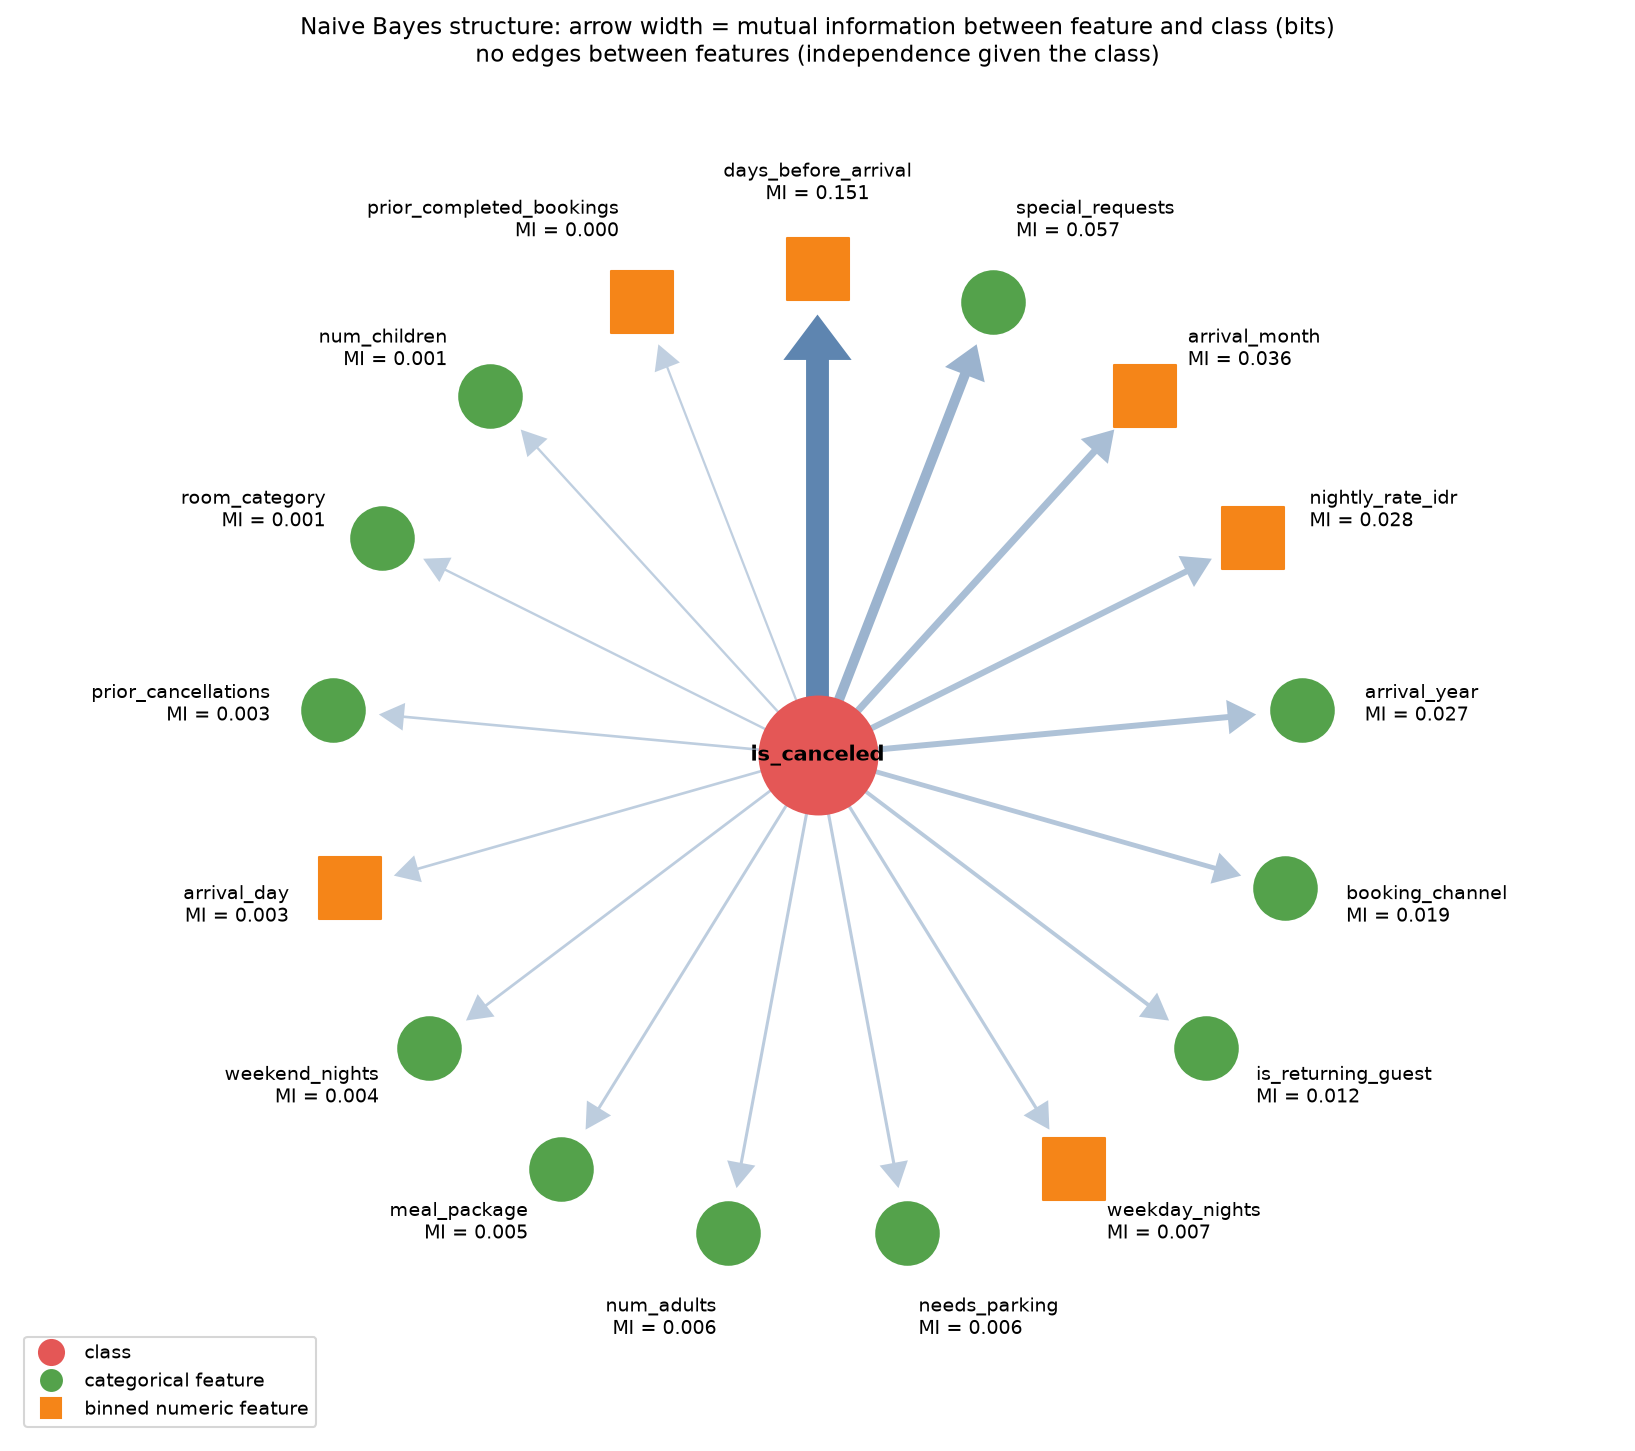
\includegraphics[width=0.78\textwidth]{output/naive_bayes_graph.png}
    \caption{Graf struktur \textit{Naive Bayes}. Lingkaran hijau adalah fitur kategorikal dan persegi jingga adalah fitur numerik yang didiskretisasi.}
    \label{fig:nb-graph}
\end{figure}

\subsection{Perbandingan Antarmodel}
Tabel~\ref{tab:ringkasan} merangkum seluruh konfigurasi pada data validasi yang sama. Semua model melampaui baseline 0,6723 dengan selisih lebar.

\begin{table}[htbp]
    \centering
    \footnotesize
    \setlength{\tabcolsep}{4pt}
    \begin{tabular}{@{}l c r r r r r@{}}
        \toprule
        Model & \textit{Submission} & Akurasi & Presisi & \textit{Recall} & F1 & ROC-AUC \\
        \midrule
        KNN ($k=15$, Manhattan, \textit{distance}) & ya & \textbf{0,8489} & \textbf{0,7998} & 0,7191 & \textbf{0,7573} & \textbf{0,9106} \\
        DTL C4.5 & ya & 0,8451 & 0,7877 & \textbf{0,7219} & 0,7533 & 0,8980 \\
        \textit{Logistic regression} L1 & & 0,7956 & 0,7433 & 0,5747 & 0,6482 & 0,8507 \\
        \textit{Logistic regression} L2 & & 0,7965 & 0,7374 & 0,5886 & 0,6547 & 0,8538 \\
        \textit{Logistic regression} Elastic Net & ya & 0,7980 & 0,7436 & 0,5853 & 0,6550 & 0,8527 \\
        SVM linear (4.000) & & 0,7934 & 0,7310 & 0,5847 & 0,6497 & 0,8510 \\
        SVM polinomial (4.000) & ya & 0,8113 & 0,7678 & 0,6081 & 0,6787 & 0,8660 \\
        SVM Gaussian (4.000) & & 0,8100 & 0,7697 & 0,5998 & 0,6742 & 0,8597 \\
        SVM Gaussian (12.000) & & 0,8268 & 0,7921 & 0,6394 & 0,7076 & 0,8784 \\
        \textit{Naive Bayes} & ya & 0,7784 & 0,6788 & 0,6148 & 0,6452 & 0,8364 \\
        \midrule
        Baseline kelas mayoritas & & 0,6723 & -- & 0 & 0 & 0,5000 \\
        \bottomrule
    \end{tabular}
    \caption{Ringkasan kinerja seluruh konfigurasi pada data validasi.}
    \label{tab:ringkasan}
\end{table}

Model terbagi ke dalam tiga kelompok yang jelas. KNN dan DTL berada di urutan teratas dengan akurasi sekitar 0,845--0,849 dan \textit{recall} di atas 0,72. Keduanya adalah model nonparametrik yang mampu membentuk batas keputusan lokal dan menangkap interaksi antarfitur. SVM berkernel menempati posisi tengah. Kemampuannya membentuk batas tidak linear dibatasi oleh subsampel. \textit{Logistic regression}, SVM linear, dan \textit{Naive Bayes} berada di urutan bawah. Dua yang pertama dibatasi oleh bentuk linear, sedangkan \textit{Naive Bayes} dibatasi oleh asumsi kebebasan bersyarat yang dilanggar oleh fitur yang saling berkaitan.

Kesalahan yang paling membedakan model adalah \textit{false negative}. Semua model memiliki tingkat FP di bawah 0,15, tetapi tingkat FN berkisar dari 0,28 untuk KNN dan DTL hingga 0,43 untuk \textit{logistic regression} L1. Model linear cenderung memprediksi kelas mayoritas pada kasus yang ambigu, sehingga banyak pembatalan tidak terdeteksi.

\subsection{Perbandingan dengan \textit{scikit-learn}}
Tabel~\ref{tab:sklearn} membandingkan setiap implementasi \textit{from scratch} dengan pembandingnya pada data latih dan validasi yang sama.

\begin{table}[htbp]
    \centering
    \small
    \setlength{\tabcolsep}{4pt}
    \begin{tabularx}{\textwidth}{@{}l l r r r r X@{}}
        \toprule
        Model & Implementasi & Akurasi & F1 & ROC-AUC & & Keterangan \\
        \midrule
        KNN & \textit{scratch} & 0,8489 & 0,7573 & 0,9106 & & \multirow{2}{=}{Identik pada empat desimal.} \\
            & \texttt{KNeighborsClassifier} & 0,8489 & 0,7573 & 0,9106 & & \\
        DTL & C4.5 \textit{scratch} & 0,8451 & 0,7533 & 0,8980 & & \multirow{2}{=}{Algoritma \textit{split} berbeda.} \\
            & \texttt{DecisionTreeClassifier} & 0,8446 & 0,7582 & 0,9016 & & \\
        LR L1 & \textit{scratch} & 0,7956 & 0,6482 & 0,8507 & & \multirow{2}{=}{Selisih koefisien maks. 0,0201.} \\
            & \texttt{LogisticRegression} & 0,7962 & 0,6493 & 0,8506 & & \\
        LR L2 & \textit{scratch} & 0,7965 & 0,6547 & 0,8538 & & \multirow{2}{=}{Selisih koefisien maks. 0,0100.} \\
            & \texttt{LogisticRegression} & 0,7969 & 0,6553 & 0,8538 & & \\
        LR EN & \textit{scratch} & 0,7980 & 0,6550 & 0,8527 & & \multirow{2}{=}{Selisih koefisien maks. 0,0142.} \\
            & \texttt{LogisticRegression} & 0,7980 & 0,6550 & 0,8527 & & \\
        SVM RBF & \textit{scratch} (12.000) & 0,8268 & 0,7076 & 0,8784 & & \multirow{2}{=}{ROC-AUC sama, kalibrasi berbeda.} \\
            & \texttt{SVC} (12.000) & 0,8263 & 0,7062 & 0,8784 & & \\
        NB & \textit{scratch} & 0,7784 & 0,6452 & 0,8364 & & \multirow{2}{=}{Beda perlakuan nilai hilang.} \\
            & \texttt{CategoricalNB} & 0,7790 & 0,6460 & 0,8344 & & \\
        \bottomrule
    \end{tabularx}
    \caption{Perbandingan implementasi \textit{from scratch} dengan \textit{scikit-learn}.}
    \label{tab:sklearn}
\end{table}

Implementasi KNN menghasilkan metrik yang identik dengan \texttt{KNeighborsClassifier} pada parameter yang sama, sehingga perhitungan jarak, pemilihan tetangga, dan pembobotan dapat dianggap benar. Implementasi \textit{logistic regression} menghasilkan metrik yang hampir sama dengan \textit{solver} SAGA setelah skala penalti disesuaikan. Selisih koefisien terbesar 0,0201 berasal dari kriteria berhenti yang berbeda, bukan dari fungsi tujuan.

Untuk SVM, pembanding \texttt{SVC} dilatih pada subsampel yang sama. Tanda fungsi keputusan kedua implementasi cocok pada 99,89\% (linear) hingga 100\% (polinomial dan Gaussian) baris validasi, dan jumlah \textit{support vector} hanya berbeda paling banyak dua. Pada eksperimen 12.000 baris, ROC-AUC keduanya sama hingga empat desimal. Selisih akurasi muncul karena \texttt{SVC} mengalibrasi peluang dengan validasi silang internal, sedangkan implementasi kelompok memakai baris di luar subsampel.

Untuk \textit{Naive Bayes}, uji ekuivalensi dengan kode kategori dan interval yang disamakan menghasilkan selisih peluang maksimum $6{,}5\times10^{-15}$ dan prediksi 100\% sama pada baris tanpa nilai hilang. Perbedaan kecil pada alur lengkap berasal dari prapemrosesan. Model kelompok melewati fitur yang hilang, sedangkan pembanding mengodekannya sebagai kategori tersendiri. Pada validasi silang, rata-rata akurasi keduanya 0,7812 dan 0,7810.

Implementasi DTL tidak dapat dibandingkan secara identik. Pembanding \texttt{DecisionTreeClassifier} hanya membentuk pohon biner, tidak mendukung atribut kategorikal secara langsung, dan memakai \textit{cost-complexity pruning} alih-alih aturan C4.5. Dengan \texttt{criterion='entropy'} dan \texttt{ccp\_alpha=0.001} sebagai padanan C4.5, akurasi keduanya berdekatan (0,8451 dan 0,8446). Pembanding memiliki \textit{recall} dan ROC-AUC sedikit lebih tinggi karena pemangkasan menghasilkan peluang daun yang lebih halus.

\subsection{Analisis Kesalahan}
Tabel~\ref{tab:error} memperlihatkan \textit{confusion matrix} kelima konfigurasi pengumpulan. KNN dan DTL memiliki jumlah FN paling sedikit, sedangkan \textit{Naive Bayes} memiliki FP paling banyak (522) karena peluangnya kurang terkalibrasi.

\begin{table}[htbp]
    \centering
    \small
    \begin{tabular}{@{}l r r r r r r@{}}
        \toprule
        Model & TN & FP & FN & TP & Tingkat FP & Tingkat FN \\
        \midrule
        KNN & 3.358 & 323 & 504 & 1.290 & 0,0877 & 0,2809 \\
        DTL C4.5 & 3.332 & 349 & 499 & 1.295 & 0,0948 & 0,2781 \\
        LR Elastic Net & 3.319 & 362 & 744 & 1.050 & 0,0983 & 0,4147 \\
        SVM polinomial & 3.351 & 330 & 703 & 1.091 & 0,0896 & 0,3919 \\
        SVM Gaussian (12.000) & 3.380 & 301 & 647 & 1.147 & 0,0818 & 0,3606 \\
        \textit{Naive Bayes} & 3.159 & 522 & 691 & 1.103 & 0,1418 & 0,3852 \\
        \bottomrule
    \end{tabular}
    \caption{\textit{Confusion matrix} pada data validasi (ambang 0,5).}
    \label{tab:error}
\end{table}

Analisis per kelompok fitur pada DTL menunjukkan bahwa kesalahan sangat bergantung pada \texttt{days\_before\_arrival}. Pada pemesanan paling lama tujuh hari sebelum kedatangan, model melewatkan 42 dari 69 pembatalan (tingkat FN 60,9\%). Pembatalan pada rentang ini jarang terjadi, sehingga daun pohon didominasi kelas tidak batal. Sebaliknya, pada rentang lebih dari 90 hari, model hanya melewatkan 151 dari 1.072 pembatalan (14,1\%), tetapi tingkat FP-nya tertinggi, yaitu 16,3\%. Pola serupa terlihat pada kanal Corporate, dengan tingkat FN 51,6\% karena pembatalan pada kanal ini jarang terjadi. Dengan kata lain, model mengandalkan rasio pembatalan dasar setiap kelompok, sehingga pembatalan pada kelompok yang jarang batal sulit dideteksi.

\subsection{\textit{Cost-Sensitive Classification}}
Pada persoalan ini, FP berarti model memprediksi batal padahal tamu datang. Jika kamar tersebut dijual ulang, hotel mengalami \textit{overbooking}, sehingga FP dianggap dua kali lebih mahal daripada FN. Penanganan berubah pada tiga hal. Pertama, aturan keputusan memakai ambang sekitar 2/3 sesuai Persamaan~\ref{eq:cost-threshold}, bukan 0,5. Kedua, kriteria pemilihan ambang adalah biaya total $2\,FP+FN$, bukan akurasi atau F1. Ketiga, ukuran yang dilaporkan adalah biaya bersama presisi dan \textit{recall}. Model tidak perlu dilatih ulang.

\begin{lstlisting}[emph={threshold_curve,fit_threshold_proba},caption={Pencarian ambang dengan biaya minimum (\texttt{src/cost\_sensitive.py})},label={lst:cost}]
def threshold_curve(proba, y, cost_fp=2.0, cost_fn=1.0):
    values, inverse = np.unique(proba, return_inverse=True)
    positives = np.bincount(inverse, weights=y, minlength=len(values))
    negatives = np.bincount(inverse, weights=1 - y, minlength=len(values))
    thresholds = np.concatenate([[values[0]], (values[:-1] + values[1:]) / 2,
                                 [np.nextafter(values[-1], np.inf)]])
    missed = np.concatenate([[0.0], np.cumsum(positives)])                 # FN
    false_alarms = negatives.sum() - np.concatenate([[0.0], np.cumsum(negatives)])  # FP
    return thresholds, cost_fp * false_alarms + cost_fn * missed
\end{lstlisting}

Fungsi \texttt{threshold\_curve} menghitung biaya untuk setiap ambang kandidat sekaligus dengan jumlah kumulatif, lalu \texttt{fit\_threshold\_proba} memilih ambang berbiaya minimum. Bila beberapa ambang memiliki biaya sama, dipilih yang paling dekat dengan 2/3. Karena ambang dicari pada data validasi yang sama dengan data penilaian, kelompok juga menghitung estimasi \textit{cross-fit}, yaitu ambang dicari pada separuh data validasi lalu dinilai pada separuh lainnya, dan sebaliknya.

\begin{table}[htbp]
    \centering
    \small
    \setlength{\tabcolsep}{3.5pt}
    \resizebox{\textwidth}{!}{%
    \begin{tabular}{@{}l r r r r r r r r r@{}}
        \toprule
        & & \multicolumn{3}{c}{Ambang 0,5} & \multicolumn{3}{c}{Ambang hasil pencarian} & & \\
        \cmidrule(lr){3-5}\cmidrule(lr){6-8}
        Model & $\tau^*$ & FP & FN & Biaya & FP & FN & Biaya & Biaya $\tau=2/3$ & Hemat \textit{cross-fit} \\
        \midrule
        KNN & 0,660 & 323 & 504 & 1.150 & 134 & 765 & \textbf{1.033} & 1.038 & 8,70\% \\
        DTL C4.5 & 0,667 & 349 & 499 & 1.197 & 225 & 685 & 1.135 & 1.137 & 3,43\% \\
        LR Elastic Net & 0,603 & 362 & 744 & 1.468 & 192 & 985 & 1.369 & 1.414 & 5,79\% \\
        SVM polinomial & 0,606 & 330 & 703 & 1.363 & 201 & 859 & 1.261 & 1.275 & 6,53\% \\
        SVM Gaussian (12.000) & 0,737 & 301 & 647 & 1.249 & 120 & 922 & 1.162 & 1.169 & 5,76\% \\
        \textit{Naive Bayes} & 0,669 & 522 & 691 & 1.735 & 194 & 975 & 1.363 & 1.367 & 20,75\% \\
        \bottomrule
    \end{tabular}}
    \caption{Biaya total $2\,FP+FN$ sebelum dan sesudah penyesuaian ambang pada data validasi.}
    \label{tab:cost}
\end{table}

Tabel~\ref{tab:cost} menunjukkan bahwa ambang 0,5 selalu lebih mahal daripada ambang hasil pencarian. Penghematan biaya pada data validasi berkisar 5,2\% (DTL) hingga 21,4\% (\textit{Naive Bayes}), dan estimasi \textit{cross-fit} tetap positif untuk semua model, yaitu 3,4\% hingga 20,8\%. Pada KNN, FP turun dari 323 menjadi 134 (58,5\%), sedangkan FN naik dari 504 menjadi 765. Presisi naik dari 0,7998 menjadi 0,8848, sedangkan \textit{recall} turun dari 0,7191 menjadi 0,5736. Model menjadi lebih berhati-hati menandai pemesanan sebagai batal, sehingga risiko \textit{overbooking} berkurang dengan konsekuensi lebih banyak pembatalan yang tidak terdeteksi.

Ambang hasil pencarian mendekati 2/3 pada delapan dari sepuluh konfigurasi, dan aturan teoretis $\tau=2/3$ hampir sama baiknya. Selisih biaya terbesar hanya 45 pada \textit{logistic regression} Elastic Net. \textit{Naive Bayes} paling diuntungkan karena peluangnya cenderung ekstrem akibat asumsi kebebasan. Dengan ambang 0,5 biayanya tertinggi, tetapi setelah penyesuaian biayanya setara dengan \textit{logistic regression}. Gambar~\ref{fig:cost} memperlihatkan bahwa setiap kurva biaya membentuk lembah datar di sekitar ambang 0,6--0,75, sedangkan ambang 0,5 masih berada di sisi yang menurun. Kurva KNN dan DTL berbentuk tangga karena peluang keduanya hanya mengambil sedikit nilai berbeda.

\begin{figure}[htbp]
    \centering
    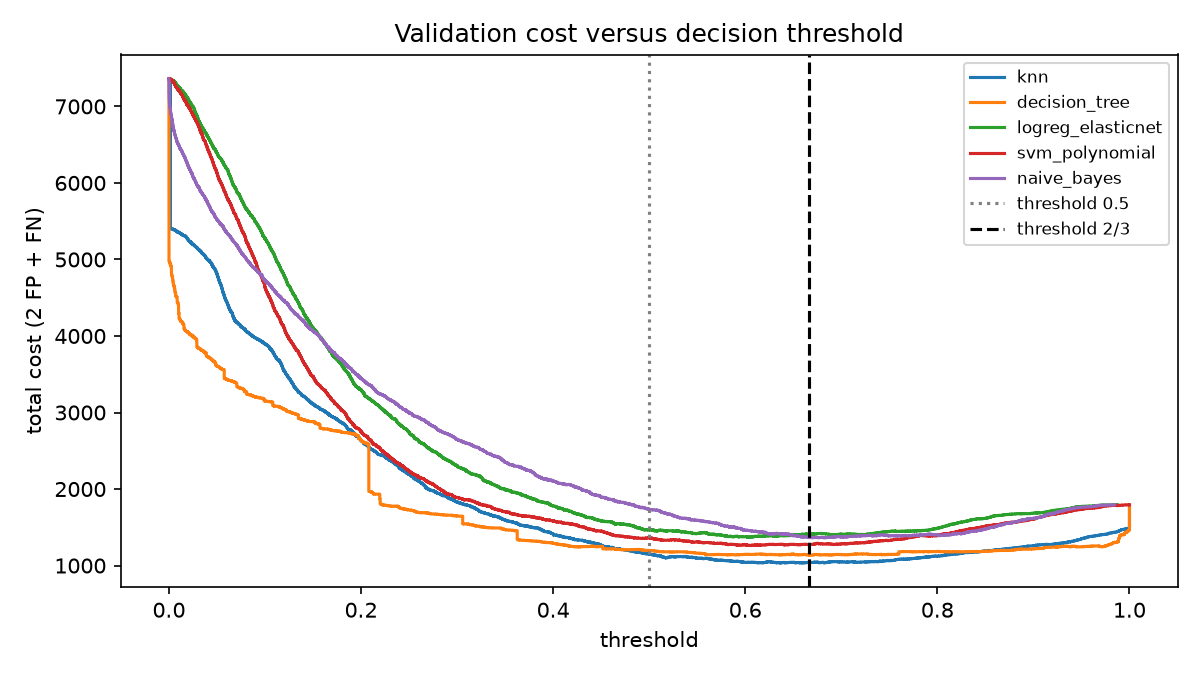
\includegraphics[width=0.85\textwidth]{output/cost_vs_threshold.png}
    \caption{Biaya total validasi terhadap ambang keputusan untuk lima konfigurasi pengumpulan.}
    \label{fig:cost}
\end{figure}

\subsection{Visualisasi Model}
\subsubsection{Video Kontur \textit{Log-Loss}}
Agar \textit{loss} hanya bergantung pada dua parameter, model dilatih pada satu fitur, yaitu \texttt{days\_before\_arrival} terstandardisasi, tanpa regularisasi, dengan laju belajar 0,05 selama 300 \textit{epoch}. Metode \texttt{plot\_loss\_contour\_video} menghitung \textit{log-loss} pada kisi $(\theta_0,\theta_1)$, menggambar konturnya, lalu menganimasikan lintasan parameter dari \texttt{history\_}. Video disimpan sebagai \path{output/lr_loss_contour.mp4}. Gambar~\ref{fig:lr-video} menampilkan bingkai terakhir. Lintasan bergerak dari $(0,0)$ dengan \textit{log-loss} 0,6931 menuju $(\theta_0,\theta_1)=(-0{,}7457;\,0{,}9001)$ dengan \textit{log-loss} 0,5400. Lintasan tegak lurus terhadap kontur, sesuai sifat \textit{gradient descent}, dan langkahnya memendek ketika mendekati minimum karena gradien mengecil.

\begin{figure}[htbp]
    \centering
    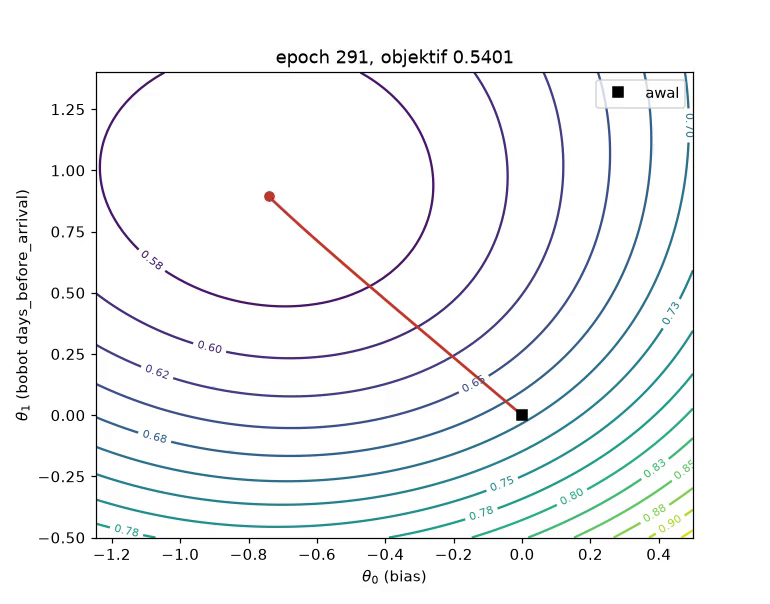
\includegraphics[width=0.62\textwidth]{figures/lr_loss_contour_last.png}
    \caption{Bingkai terakhir video kontur \textit{log-loss} dan lintasan parameter.}
    \label{fig:lr-video}
\end{figure}

\subsubsection{Bidang Pemisah SVM}
Visualisasi memakai fitur \texttt{days\_before\_arrival} dan \texttt{nightly\_rate\_idr} hasil \textit{preprocessing}. Setiap kernel dilatih dengan $C=1$ pada subsampel berstrata 2.000 baris. Garis utuh menyatakan batas keputusan $f(\mathbf{x})=0$, garis putus-putus menyatakan margin $f(\mathbf{x})=\pm1$, dan lingkaran hitam menandai \textit{support vector}. Kernel linear menghasilkan garis lurus dengan 1.158 \textit{support vector}, polinomial menghasilkan kurva dengan 1.089, dan Gaussian menghasilkan daerah tertutup yang lebih lokal dengan 1.063 \textit{support vector}. Pada ketiga gambar, kedua kelas sangat bertumpang tindih di bidang dua fitur ini, sehingga lebih dari separuh sampel menjadi \textit{support vector}.

\begin{figure}[htbp]
    \centering
    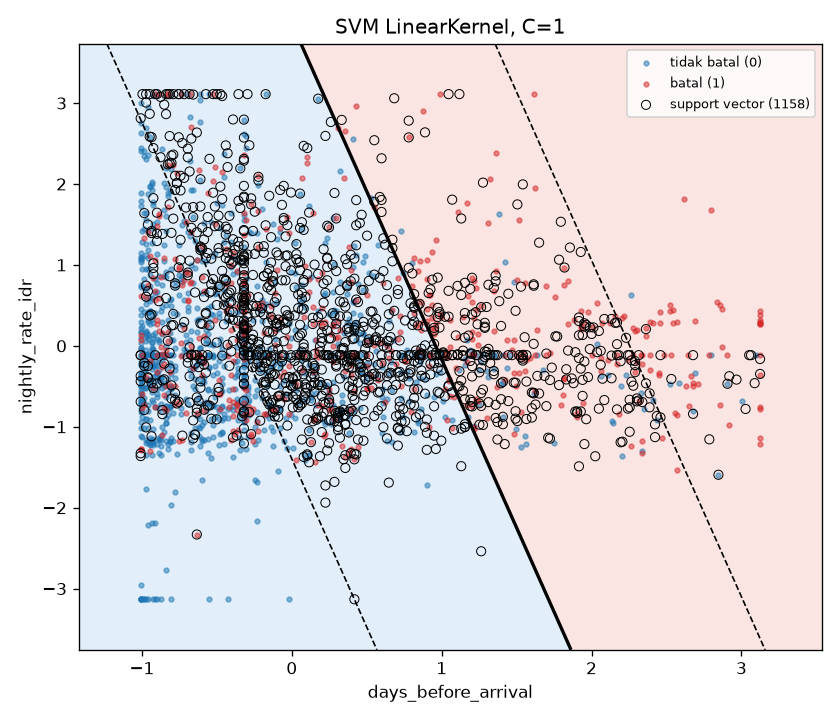
\includegraphics[width=0.32\textwidth]{output/svm_boundary_linear.png}\hfill
    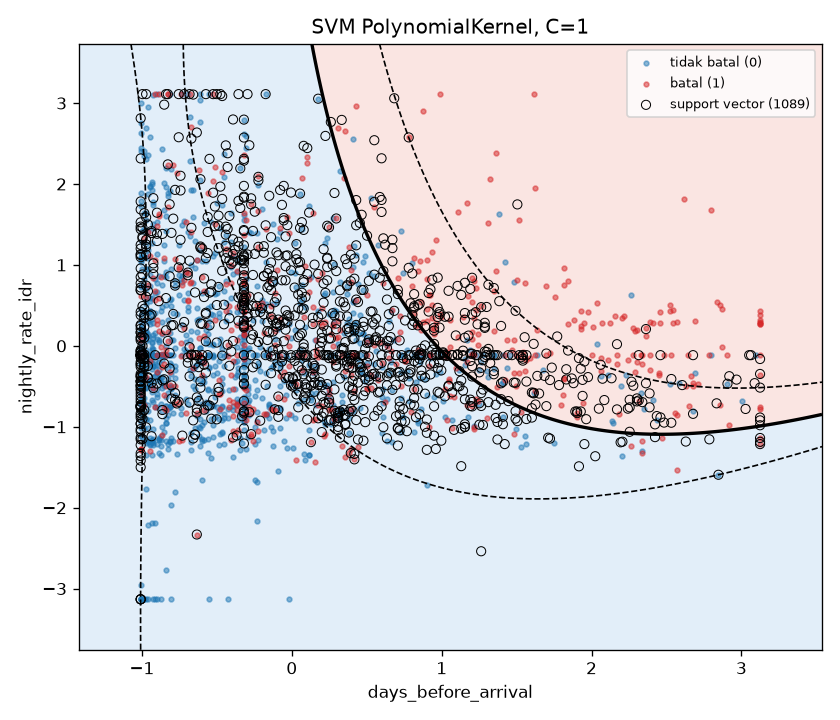
\includegraphics[width=0.32\textwidth]{output/svm_boundary_polynomial.png}\hfill
    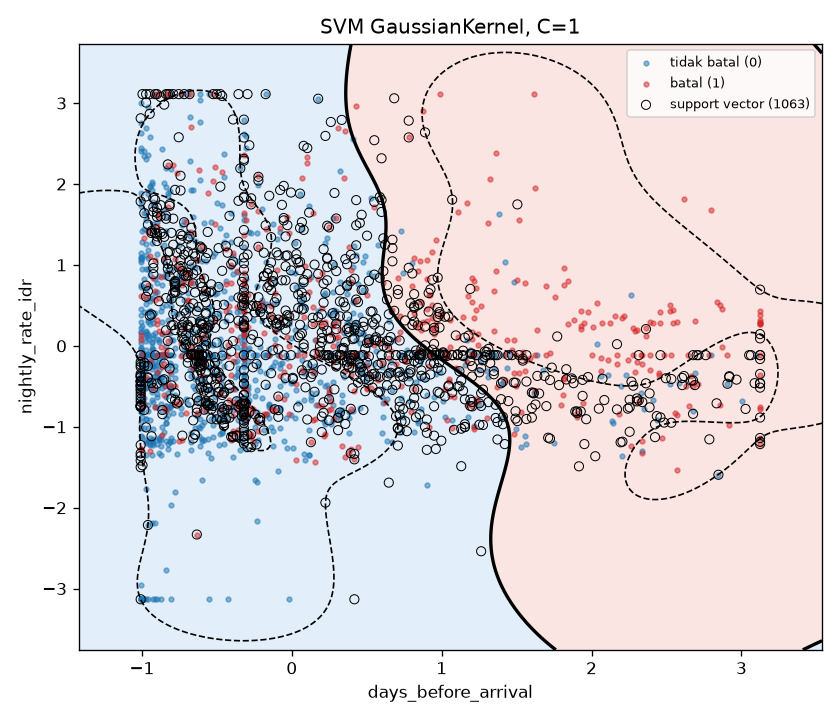
\includegraphics[width=0.32\textwidth]{output/svm_boundary_gaussian.png}
    \caption{Bidang pemisah, margin, dan \textit{support vector} untuk kernel linear, polinomial, dan Gaussian.}
    \label{fig:svm-boundary}
\end{figure}

\subsection{Algoritma Optimasi Model}
\subsubsection{FISTA dan Adam pada \textit{Logistic Regression}}
Eksperimen ini membandingkan kecepatan konvergensi \textit{gradient descent} (GD) proksimal, FISTA, dan Adam pada konfigurasi regularisasi baku ($\alpha=0{,}01$, \texttt{l1\_ratio}=0,5). Setiap \textit{optimizer} dijalankan 1.000 \textit{epoch} dengan \textit{batch} penuh dan tanpa kriteria berhenti dini. Objektif referensi adalah objektif terkecil dari FISTA yang dijalankan 20.000 \textit{epoch}. Tabel~\ref{tab:optim-lr} mencatat \textit{epoch} pertama saat objektif berada dalam $10^{-3}$ dan $10^{-4}$ dari referensi. Adam hanya diuji pada penalti L2 karena implementasinya terbatas pada fungsi tujuan yang mulus. Ukuran langkah FISTA $1/L$ bernilai sekitar 1,03 untuk kedua penalti.

\begin{table}[htbp]
    \centering
    \small
    \begin{tabular}{@{}l l r r r r r@{}}
        \toprule
        Penalti & \textit{Optimizer} & \multicolumn{2}{c}{\textit{Epoch} hingga} & Objektif akhir & Akurasi & Bobot nol \\
        \cmidrule(lr){3-4}
         & & $10^{-3}$ & $10^{-4}$ & & validasi & \\
        \midrule
        \multirow{3}{*}{Elastic Net} & GD, $\eta=0{,}1$ & 301 & 539 & 0,464751 & 0,7978 & 18 \\
         & GD, $\eta=0{,}5$ & 59 & 107 & 0,464746 & 0,7980 & 19 \\
         & FISTA, $\eta=1/L$ & \textbf{10} & \textbf{20} & 0,464746 & 0,7980 & 19 \\
        \midrule
        \multirow{4}{*}{L2} & GD, $\eta=0{,}1$ & 297 & 542 & 0,450102 & 0,7965 & 0 \\
         & GD, $\eta=0{,}5$ & 59 & 107 & 0,450093 & 0,7969 & 0 \\
         & FISTA, $\eta=1/L$ & \textbf{9} & \textbf{20} & 0,450093 & 0,7969 & 0 \\
         & Adam, $\eta=0{,}05$ & 27 & 67 & 0,450093 & 0,7969 & 0 \\
        \bottomrule
    \end{tabular}
    \caption{Kecepatan konvergensi GD, FISTA, dan Adam pada \textit{logistic regression} (1.000 \textit{epoch}).}
    \label{tab:optim-lr}
\end{table}

Semua \textit{optimizer} mencapai objektif yang sama hingga enam desimal, kecuali GD dengan laju baku 0,1 yang masih tertinggal sekitar $5\times10^{-6}$ setelah 1.000 \textit{epoch}. Akurasi validasi dan jumlah bobot nol juga sama, sehingga FISTA dan Adam tidak mengubah solusi, melainkan mempercepat jalan menuju solusi tersebut. FISTA paling cepat. FISTA membutuhkan 10 \textit{epoch} untuk mencapai jarak $10^{-3}$ pada Elastic Net, yaitu 30 kali lebih cepat daripada GD dengan laju baku dan hampir 6 kali lebih cepat daripada GD dengan laju 0,5 yang telah disetel. Keunggulan ini tidak memerlukan penyetelan laju belajar, karena $1/L$ dihitung langsung dari data. Adam pada penalti L2 membutuhkan 27 \textit{epoch}, sekitar dua kali lebih cepat daripada GD yang disetel, tetapi masih tiga kali lebih lambat daripada FISTA. Pada \textit{batch} penuh, momentum Nesterov dengan ukuran langkah yang tepat lebih efektif daripada laju belajar adaptif per parameter.

\subsubsection{\textit{Cost-Complexity Pruning} pada DTL}
\texttt{PrunedDecisionTree} pada \path{src/dtl_tuning.py} memangkas pohon C4.5 yang telah dilatih menggunakan kriteria Persamaan~\ref{eq:ccp}. Fungsi \texttt{prune\_node} bekerja dari daun ke akar. Subpohon diganti daun apabila galat kelas mayoritas sebagai daun ditambah $\alpha$ tidak melebihi jumlah biaya daun-daun subpohon tersebut. Kelas ini juga dapat memilih $k$ fitur teratas menurut \textit{mutual information} yang dihitung dari tabel peluang \textit{Naive Bayes} pada data latih lipatan.

\begin{lstlisting}[emph={prune_node},caption={Pemangkasan \textit{cost-complexity} (\texttt{src/dtl\_tuning.py})},label={lst:prune}]
def prune_node(node, alpha, total):
    counts = node.class_counts
    leaf_cost = min(counts[0], counts[1]) / total + alpha
    if node.is_leaf():
        return leaf_cost, node
    children, subtree_cost = {}, 0.0
    for key, child in node.children.items():
        cost, new_child = prune_node(child, alpha, total)
        children[key] = new_child
        subtree_cost += cost
    if leaf_cost <= subtree_cost:
        return leaf_cost, TreeNode(counts, node.n_samples, node.depth)
    return subtree_cost, replace(node, children=children)
\end{lstlisting}

Tabel~\ref{tab:prune} menyajikan validasi silang lima lipatan untuk dua konfigurasi: pohon baku dengan fitur turunan, serta konfigurasi \texttt{BEST} pada kode, yaitu fitur asli, 14 fitur teratas, dan \texttt{min\_gain}=$10^{-4}$. Pemangkasan ringan dengan $\alpha=5\times10^{-5}$ menaikkan akurasi kedua konfigurasi sekitar 0,35--0,4 poin persentase. Nilai $\alpha$ yang lebih besar menurunkan kinerja dengan cepat, karena pohon kehilangan aturan yang masih berguna. Konfigurasi \texttt{BEST} dengan $\alpha=5\times10^{-5}$ mencapai akurasi validasi silang 0,8506. Pada pembagian validasi utama, konfigurasi ini memperoleh akurasi 0,8552, F1 0,7639, dan ROC-AUC 0,9101, naik 1,0 poin persentase dari pohon C4.5 tanpa pemangkasan. Ukuran pohon menyusut dari 5.033 menjadi 820 simpul, sehingga model juga jauh lebih mudah ditafsirkan. Kenaikan ini muncul karena cabang-cabang dalam yang hanya mengikuti derau digantikan daun dengan distribusi kelas yang lebih stabil. CSV \path{output/submission_dtl_tuned.csv} dapat direproduksi persis dari konfigurasi ini.

\begin{table}[htbp]
    \centering
    \small
    \begin{tabular}{@{}l r r r r r@{}}
        \toprule
        Konfigurasi & $\alpha$ & Akurasi & F1 & ROC-AUC & Std. akurasi \\
        \midrule
        Baku (fitur turunan, semua fitur) & 0 & 0,8461 & 0,7542 & 0,8971 & 0,0041 \\
         & $2\times10^{-5}$ & 0,8480 & 0,7556 & 0,8989 & 0,0033 \\
         & $5\times10^{-5}$ & 0,8496 & 0,7549 & 0,9054 & 0,0042 \\
         & $10^{-4}$ & 0,8487 & 0,7504 & 0,8945 & 0,0044 \\
         & $10^{-3}$ & 0,8196 & 0,6983 & 0,8351 & 0,0049 \\
        \midrule
        \texttt{BEST} (fitur asli, 14 fitur) & 0 & 0,8467 & 0,7554 & 0,8968 & 0,0010 \\
         & $2\times10^{-5}$ & 0,8486 & 0,7564 & 0,8983 & 0,0005 \\
         & $5\times10^{-5}$ & \textbf{0,8506} & \textbf{0,7569} & \textbf{0,9065} & 0,0031 \\
         & $10^{-4}$ & 0,8494 & 0,7520 & 0,8996 & 0,0029 \\
         & $10^{-3}$ & 0,8193 & 0,6985 & 0,8293 & 0,0055 \\
        \bottomrule
    \end{tabular}
    \caption{Validasi silang lima lipatan DTL dengan berbagai nilai $\alpha$ pemangkasan.}
    \label{tab:prune}
\end{table}

\subsubsection{\textit{Random Search} dan Pembobotan Kolom pada KNN}
KNN baku memberi bobot yang sama kepada setiap kolom, sehingga kolom yang hampir tidak informatif ikut menentukan jarak. \texttt{WeightedKNN} pada \path{src/knn_tuning.py} mengalikan setiap kolom dengan bobot $w_j=(I_j/I_{\max})^{\gamma}$, dengan $I_j$ \textit{mutual information} kolom $j$ terhadap target yang dihitung dari data latih lipatan. Pada jarak Minkowski orde $p$, mengalikan kolom dengan $w_j$ setara dengan memberi bobot $w_j^{\,p}$ pada selisih kolom tersebut. Kelas ini juga dapat membuang kolom di luar \texttt{top\_k} teratas dan mengecilkan bobot kolom \textit{one-hot}. Model tetap berupa satu KNN, bukan \textit{ensemble}.

\begin{lstlisting}[emph={column_scale},caption={Bobot kolom berbasis \textit{mutual information} (\texttt{src/knn\_tuning.py})},label={lst:knn-weight}]
def column_scale(mi, names, gamma=0.0, top_k=0, onehot_factor=1.0):
    weight = np.ones(len(mi)) if gamma == 0 or mi.max() <= 0 else (mi / mi.max()) ** gamma
    if top_k:
        keep = np.zeros(len(mi))
        keep[np.argsort(-mi, kind="stable")[:top_k]] = 1
        weight = weight * keep
    onehot = np.array(["=" in str(n) for n in names])
    return np.where(onehot, weight * onehot_factor, weight)
\end{lstlisting}

Ruang pencarian mencakup jenis \textit{scaler}, pengodean siklik bulan ($\sin$ dan $\cos$), transformasi log untuk fitur miring, metrik jarak, $\gamma$, \texttt{top\_k}, faktor \textit{one-hot}, $k$, dan pembobotan tetangga. Ruang ini terlalu besar untuk \textit{grid search}, sehingga digunakan \textit{random search}. Pencarian memakai konfigurasi baku ditambah 30 konfigurasi acak dengan \texttt{seed=42}, dan setiap konfigurasi dievaluasi pada sembilan nilai $k$ dan dua pembobotan dengan validasi silang lima lipatan. Total terdapat 558 kombinasi. Seluruh langkah yang belajar dari data, termasuk \textit{mutual information}, di-\textit{fit} ulang di dalam setiap lipatan.

\begin{table}[htbp]
    \centering
    \small
    \setlength{\tabcolsep}{4pt}
    \begin{tabularx}{\textwidth}{@{}X r r r r r@{}}
        \toprule
        Konfigurasi & Akurasi CV & Std. & F1 CV & ROC-AUC CV & Akurasi validasi \\
        \midrule
        KNN baku (standar, Manhattan, $k=15$, \textit{distance}) & 0,8429 & 0,0016 & 0,7484 & 0,9049 & 0,8489 \\
        Terbaik: min-max, bulan siklik, Manhattan, $\gamma=0{,}5$, \texttt{top\_k}=24, $k=15$, \textit{distance} & \textbf{0,8612} & 0,0044 & \textbf{0,7809} & \textbf{0,9229} & \textbf{0,8639} \\
        \bottomrule
    \end{tabularx}
    \caption{Hasil \textit{random search} KNN dengan validasi silang lima lipatan.}
    \label{tab:knn-tune}
\end{table}

Tabel~\ref{tab:knn-tune} menunjukkan bahwa konfigurasi terbaik menaikkan akurasi validasi silang dari 0,8429 menjadi 0,8612 dan F1 dari 0,7484 menjadi 0,7809. Pada pembagian validasi utama, akurasinya 0,8639, sehingga KNN berbobot kolom lebih baik daripada seluruh konfigurasi sebelumnya. Enam konfigurasi teratas sama-sama memakai \textit{scaler} min-max, jarak Manhattan, $\gamma=0{,}5$, dan 24 kolom teratas. Pola ini menunjukkan bahwa sumber kenaikan terutama adalah pengurangan pengaruh kolom lemah pada jarak, bukan nilai $k$. \textit{Scaler} min-max juga membatasi setiap fitur pada rentang $[0,1]$, sehingga kolom \textit{one-hot} dan kolom numerik memiliki skala yang setara. Pencarian ini dijalankan ulang saat penyusunan laporan. CSV yang dihasilkan sama dengan \path{output/submission_knn_tuned.csv} pada 93,9\% baris, sehingga berkas tersebut kemungkinan berasal dari putaran pencarian yang berbeda.

\subsubsection{Penalti MDL pada Atribut Numerik DTL}
\texttt{MDLDecisionTree} pada \path{src/dtl_tuning.py} menurunkan kelas \texttt{DecisionTree} dan hanya mengganti pencarian ambang numerik. \textit{Gain} setiap kandidat ambang dikurangi $\log_2(N-1)/|D|$ seperti pada dasar teori, dengan $N-1$ jumlah kandidat ambang dan $|D|$ bobot sampel yang nilainya diketahui. Ambang dipilih berdasarkan \textit{gain} yang belum dipenalti, sedangkan nilai terpenalti dipakai untuk membandingkan antaratribut. Dengan cara ini, atribut numerik dengan banyak nilai unik, seperti tarif dan \texttt{days\_before\_arrival}, tidak lagi diuntungkan secara semu dibanding atribut kategorikal.

\begin{lstlisting}[caption={Penalti MDL pada \textit{gain} ambang numerik (\texttt{src/dtl\_tuning.py}, diringkas)},label={lst:mdl}]
penalised = gain - np.log2(len(positions)) / known_w
ratios = np.divide(penalised, split_info, out=np.zeros_like(gain), where=split_info > 1e-12)
valid &= (penalised > self.min_gain) & (split_info > 1e-12)
score = gain if self.threshold_by == "gain" else ratios
best = int(np.argmax(np.where(valid, score, -np.inf)))
\end{lstlisting}

Konfigurasi terbaik memakai penalti MDL, 14 fitur teratas, \texttt{min\_gain}=$10^{-4}$, pemangkasan $\alpha=5\times10^{-5}$, serta imputasi median dan modus sebagai pengganti bobot pecahan untuk nilai hilang. Tabel~\ref{tab:mdl} menunjukkan bahwa penalti MDL saja menaikkan akurasi validasi silang dari 0,8506 menjadi 0,8530. Penambahan imputasi menaikkan akurasi lagi menjadi 0,8585 dengan simpangan baku 0,0040. Pada data ini, imputasi tampaknya membantu karena bobot pecahan menyebarkan sampel bernilai hilang ke banyak daun kecil, sedangkan imputasi mengirim sampel tersebut ke satu cabang. Ambang keputusan 0,55 pada kode memberi akurasi validasi silang yang sama dengan ambang 0,5.

\begin{table}[htbp]
    \centering
    \small
    \setlength{\tabcolsep}{4pt}
    \begin{tabularx}{\textwidth}{@{}X r r r r r@{}}
        \toprule
        Konfigurasi DTL & Akurasi CV & Std. & F1 CV & ROC-AUC CV & Akurasi validasi \\
        \midrule
        Terpangkas tanpa MDL (\texttt{BEST}) & 0,8506 & 0,0031 & 0,7569 & 0,9065 & 0,8552 \\
        Terpangkas dengan MDL, bobot pecahan & 0,8530 & 0,0052 & 0,7622 & 0,9085 & 0,8566 \\
        Terpangkas dengan MDL dan imputasi & \textbf{0,8585} & 0,0040 & \textbf{0,7732} & 0,9010 & \textbf{0,8636} \\
        \bottomrule
    \end{tabularx}
    \caption{Pengaruh penalti MDL dan imputasi pada DTL terpangkas (ambang 0,5).}
    \label{tab:mdl}
\end{table}

Pohon akhir berisi 823 simpul. CSV \path{output/submission_dtl_mdl.csv} dapat direproduksi persis dari konfigurasi ini dengan ambang 0,55.

\subsubsection{Pipeline Kombinasi pada KNN}
Eksperimen terakhir pada KNN menggabungkan beberapa temuan sebelumnya ke dalam satu pipeline. \texttt{combo\_pipeline} tidak memakai fitur turunan dan tidak memotong pencilan, mengubah bulan kedatangan menjadi pasangan $\sin$ dan $\cos$, serta memperlakukan nilai hilang pada fitur kategorikal sebagai kategori tersendiri bernama \texttt{Missing}. Perlakuan terakhir ini dipilih karena hilangnya nilai kategori dapat membawa informasi sendiri, sebagaimana terlihat pada \texttt{special\_requests}. Model yang dipakai adalah \texttt{WeightedKNN} dengan $k=15$, jarak Manhattan, bobot jarak, $\gamma=0{,}5$, dan 20 kolom teratas.

\begin{lstlisting}[caption={Pipeline kombinasi KNN (\texttt{src/knn\_tuning.py})},label={lst:knn-combo}]
COMBO = {"k": 15, "metric": "manhattan", "p": 1, "weights": "distance", "gamma": 0.5, "top_k": 20}

def missing_as_category(df, cols=("meal_package", "room_category", "booking_channel")):
    df = df.copy()
    for c in cols:
        df[c] = df[c].fillna("Missing")
    return df

def combo_pipeline():
    return PreparationPipeline([cyclic_month, missing_as_category, Imputer(),
                                CategoricalEncoder(), Scaler("standard")])
\end{lstlisting}

Konfigurasi ini mencapai akurasi validasi silang 0,8651 dengan simpangan baku 0,0050, F1 0,7864, dan ROC-AUC 0,9267. Pada pembagian validasi utama, akurasinya 0,8674, F1 0,7928, dan ROC-AUC 0,9304. Dengan hasil tersebut, KNN dengan pipeline kombinasi menjadi model tunggal terbaik pada laporan ini, sedikit di atas KNN hasil \textit{random search} (0,8612) dan DTL dengan penalti MDL (0,8585). CSV \path{output/submission_knn_combo.csv} dapat direproduksi persis dari konfigurasi ini.

\subsubsection{Diskretisasi MDL pada \textit{Naive Bayes}}
Eksperimen ini mengganti 20 interval kuantil dengan ambang Fayyad--Irani, sementara fitur, $\alpha=1$, dan perlakuan nilai hilang tetap sama. Tabel~\ref{tab:nb-mdl} membandingkan kedua cara diskretisasi dengan validasi silang lima lipatan dan pada pembagian validasi utama.

\begin{table}[htbp]
    \centering
    \small
    \begin{tabular}{@{}l l r r r r r@{}}
        \toprule
        Diskretisasi & Evaluasi & Akurasi & Presisi & \textit{Recall} & F1 & ROC-AUC \\
        \midrule
        Kuantil, 20 interval & 5 lipatan & \textbf{0,7812} & \textbf{0,6871} & 0,6099 & 0,6462 & 0,8347 \\
        MDL Fayyad--Irani & 5 lipatan & 0,7800 & 0,6822 & \textbf{0,6149} & \textbf{0,6468} & 0,8347 \\
        \midrule
        Kuantil, 20 interval & validasi & 0,7784 & 0,6788 & 0,6148 & 0,6452 & 0,8364 \\
        MDL Fayyad--Irani & validasi & \textbf{0,7808} & 0,6787 & \textbf{0,6288} & \textbf{0,6528} & \textbf{0,8379} \\
        \bottomrule
    \end{tabular}
    \caption{Perbandingan diskretisasi kuantil dan MDL pada \textit{Naive Bayes}.}
    \label{tab:nb-mdl}
\end{table}

Kedua cara memberi kinerja yang hampir sama. Pada validasi silang, selisih akurasi hanya 0,0012 dan ROC-AUC sama hingga empat desimal, sedangkan pada pembagian validasi utama MDL sedikit lebih baik. Selisih sekecil ini masih berada dalam variasi antarlipatan, karena akurasi per lipatan berkisar 0,775 hingga 0,787. Perbedaan yang lebih jelas terlihat pada jumlah interval. MDL hanya memakai 8 ambang untuk \texttt{days\_before\_arrival} dan \texttt{nightly\_rate\_idr}, 5 ambang untuk \texttt{arrival\_month}, dan 3 ambang untuk \texttt{weekday\_nights}. \texttt{arrival\_day} tidak dipotong sama sekali, sehingga fitur ini praktis tidak berpengaruh pada posterior. Perubahan terpenting terjadi pada \texttt{prior\_completed\_bookings}. Batas kuantil fitur ini runtuh di nilai 0, sehingga seluruh 21.856 baris latih masuk ke satu interval dan \textit{mutual information}-nya nol. MDL menempatkan ambang di 0,5, yang memisahkan 477 tamu dengan riwayat pemesanan dari tamu lainnya, sehingga \textit{mutual information} fitur ini naik menjadi 0,0111 bit. Kelemahan yang dibahas pada Subbab~\ref{sec:hasil-nb} dengan demikian teratasi, tetapi sumbangannya kecil karena fitur tersebut hanya positif pada sekitar 2\% baris. Model dengan interval lebih sedikit ini lebih sederhana tanpa kehilangan kinerja, tetapi tidak menutup selisih terhadap pohon dan KNN. Batas utama \textit{Naive Bayes} tetap asumsi kebebasan bersyarat.

\subsubsection{Seleksi \textit{Working Set} Orde Kedua pada SMO}
\texttt{SVMWSS2} dilatih dengan kernel, $C$, subsampel 4.000 baris, dan toleransi yang sama dengan Tabel~\ref{tab:svm}. Tabel~\ref{tab:svm-wss} membandingkan jumlah iterasi SMO dan hasil validasinya.

\begin{table}[htbp]
    \centering
    \small
    \begin{tabular}{@{}l r r c r r r@{}}
        \toprule
        Kernel & \multicolumn{2}{c}{Iterasi SMO} & Konvergen & \multicolumn{2}{c}{Waktu \textit{fit} (detik)} & Tanda keputusan \\
        \cmidrule(lr){2-3}\cmidrule(lr){5-6}
         & Orde 1 & Orde 2 & (orde 2) & Orde 1 & Orde 2 & sama \\
        \midrule
        Linear & 100.000 & \textbf{54.788} & ya & 18,4 & \textbf{11,3} & 99,89\% \\
        Polinomial ($d=3$) & 60.733 & \textbf{9.842} & ya & 13,1 & \textbf{3,8} & 100\% \\
        Gaussian & 28.242 & \textbf{8.878} & ya & 6,2 & \textbf{3,4} & 100\% \\
        \bottomrule
    \end{tabular}
    \caption{Seleksi \textit{working set} orde pertama dan orde kedua pada SMO (subsampel 4.000 baris).}
    \label{tab:svm-wss}
\end{table}

Seleksi orde kedua mengurangi jumlah iterasi 3,2 kali pada kernel Gaussian dan 6,2 kali pada kernel polinomial. Pada kernel linear, versi orde pertama berhenti di batas 100.000 iterasi tanpa konvergen, sedangkan versi orde kedua konvergen pada 54.788 iterasi. Waktu \textit{fit} turun lebih sedikit daripada jumlah iterasi karena waktu tersebut juga mencakup perhitungan matriks kernel dan \textit{Platt scaling}. Akurasi, presisi, \textit{recall}, F1, dan ROC-AUC kedua versi sama hingga empat desimal pada ketiga kernel, dan tanda nilai keputusan pada data validasi sama pada sedikitnya 99,89\% baris. Hasil ini sesuai dengan rancangannya. Kriteria berhenti tidak berubah, sehingga kedua versi mencapai solusi dual yang sama dan perbedaannya hanya pada jalan menuju solusi. Penghematan waktu ini dapat dipakai untuk melatih SVM pada subsampel yang lebih besar.

\subsection{\textit{Submission} Kaggle}
Lima CSV dihasilkan dari konfigurasi pengumpulan, masing-masing satu per algoritma, dengan proporsi prediksi batal 24,6\% hingga 28,7\%. CSV DTL C4.5 dikirim ke Kaggle dan memperoleh skor publik 0,82005. Skor ini sekitar 2,5 poin persentase di bawah akurasi validasi lokal DTL (0,8451). Selisih tersebut dapat berasal dari variasi sampel pada leaderboard publik dan dari perbedaan metrik leaderboard, karena metrik yang dipakai Kaggle tidak diketahui secara pasti. Notebook pengumpulan bersifat \textit{reproducible} karena eksekusi ulang dari sel pertama menghasilkan \path{submission_decision_tree.csv} yang identik dengan berkas pada \path{output/}.

\clearpage
\section{Kesimpulan dan Saran}
\subsection{Kesimpulan}
Persoalan prediksi pembatalan pemesanan penginapan telah diselesaikan sebagai klasifikasi biner dengan lima algoritma yang diimplementasikan \textit{from scratch} menggunakan NumPy. Seluruh model memakai antarmuka yang sama, dapat disimpan dan dimuat ulang tanpa perubahan prediksi, dan dievaluasi pada pembagian validasi yang sama. Pipeline \textit{preprocessing} di-\textit{fit} hanya pada data latih, sehingga skor validasi bebas dari \textit{data leakage}.

Berdasarkan Tabel~\ref{tab:ringkasan}, KNN dengan $k=15$, jarak Manhattan, dan bobot jarak memberikan kinerja validasi terbaik, dengan akurasi 0,8489, F1 0,7573, dan ROC-AUC 0,9106. DTL C4.5 menyusul sangat dekat dengan akurasi 0,8451 tanpa memerlukan imputasi, serta memperoleh skor publik Kaggle 0,82005. Kedua model nonparametrik ini unggul karena mampu menangkap hubungan tidak linear dan interaksi antarfitur, terutama peran \texttt{days\_before\_arrival} yang menjadi fitur paling informatif. SVM berkernel berada di posisi tengah dan dibatasi oleh subsampel, sedangkan \textit{logistic regression} dan \textit{Naive Bayes} dibatasi oleh bentuk linear dan asumsi kebebasan bersyarat.

Model akhir kelompok adalah KNN jarak Manhattan dengan $k=18$ dan bobot tetangga $1/d^{1{,}5}$ (Subbab~\ref{sec:model-akhir}). Model ini bekerja di ruang fitur yang setiap kolomnya diberi bobot dari \textit{mutual information} dan pengali per atribut, ditambah fitur tanggal dan imputasi KNN untuk \texttt{days\_before\_arrival}. Dengan kriteria \textit{macro} F1 yang dipakai Kaggle, model ini memperoleh 0,8521 pada validasi silang lima lipatan, naik dari 0,8228 untuk KNN tanpa pembobotan kolom. \textit{Submission} model ini memperoleh skor publik Kaggle 0,86239, naik dari 0,86060 pada versi sebelumnya. Hasil ini menunjukkan bahwa pada KNN, pemilihan ruang jarak lebih menentukan daripada pemilihan $k$.

Perbandingan dengan \textit{scikit-learn} menunjukkan bahwa implementasi kelompok benar. KNN dan \textit{logistic regression} menghasilkan metrik yang identik atau hampir sama, SVM menghasilkan tanda keputusan yang cocok pada sedikitnya 99,89\% baris, dan \textit{Naive Bayes} menghasilkan peluang yang sama hingga presisi mesin ketika kode masukannya disamakan.

Pada skenario \textit{cost-sensitive} dengan biaya FP dua kali FN, mengganti ambang 0,5 dengan ambang sekitar 2/3 menurunkan biaya total 5,2\% hingga 21,4\% tanpa melatih ulang model. Pada optimasi model, FISTA mempercepat konvergensi \textit{logistic regression} hingga 30 kali dan Adam hingga 11 kali tanpa mengubah solusi, seleksi \textit{working set} orde kedua mengurangi iterasi SMO 3 hingga 6 kali dengan hasil yang sama, diskretisasi MDL membuat \textit{Naive Bayes} lebih sederhana dengan kinerja setara, \textit{cost-complexity pruning} menaikkan akurasi validasi silang DTL menjadi 0,8506 sambil memperkecil pohon dari 5.033 menjadi 820 simpul, dan penalti MDL bersama imputasi menaikkannya lagi menjadi 0,8585. Pada KNN, \textit{random search} dengan pembobotan kolom berbasis \textit{mutual information} menaikkan akurasi validasi silang dari 0,8429 menjadi 0,8612, dan pipeline kombinasi dengan bulan siklik serta kategori hilang sebagai kategori tersendiri mencapai 0,8651, tertinggi di antara seluruh model.

\subsection{Saran}
Pengembangan selanjutnya dapat mencakup hal-hal berikut.
\begin{enumerate}
    \setlength{\itemsep}{0pt}
    \item Memindahkan DTL dengan penalti MDL ke dalam notebook pengumpulan agar hasilnya dapat direproduksi langsung dari notebook, seperti model akhir KNN.
    \item Melatih SVM pada data yang lebih besar melalui \textit{cache} baris kernel atau pendekatan aproksimasi kernel, karena kenaikan subsampel dari 4.000 ke 12.000 baris terbukti meningkatkan kinerja. Seleksi \textit{working set} orde kedua yang lebih cepat dapat dipakai untuk keperluan ini.
    \item Menambahkan fitur yang menangkap pola musiman, misalnya pengodean siklik untuk bulan kedatangan, serta interaksi \texttt{days\_before\_arrival} dengan tarif agar model linear dapat menangkap hubungan tidak linear.
    \item Mencoba struktur TAN pada \textit{Naive Bayes}, karena diskretisasi MDL tidak menaikkan kinerja secara berarti dan batas utamanya adalah asumsi kebebasan bersyarat.
    \item Mencari pengali bobot kolom KNN dengan validasi bersarang agar perkiraan kinerja tidak optimistis, serta menambahkan fitur baru ke dalam pencarian tersebut.
\end{enumerate}

\pagebreak
\section{Pembagian Tugas Tiap Anggota Kelompok}
Pembagian berikut disusun dari rencana kerja pada \path{SPEC.md} dan riwayat \textit{commit} repositori.
\begin{table}[ht]
    \centering
    \small
    \renewcommand{\arraystretch}{1.4}
    \begin{tabularx}{\textwidth}{@{}p{4.6cm}lX@{}}
        \toprule
        \textbf{Nama Lengkap} & \textbf{NIM} & \textbf{Tugas/Kontribusi} \\
        \midrule
        Samuelson Dharmawan Tanuraharja & 13524001 & SVM \textit{from scratch} dengan SMO, kernel linear, polinomial, dan Gaussian; strategi subsampel dan Platt scaling; perbandingan dengan SVC; visualisasi bidang pemisah. \\
        Edward David Rumahorbo & 13524036 & \textit{Naive Bayes} \textit{from scratch}; \textit{data understanding} dan perbandingan distribusi latih-uji; pembanding \texttt{CategoricalNB}; graf struktur \textit{Naive Bayes}; \textit{cost-sensitive classification}; eksperimen \textit{weighted} KNN dan pohon terpangkas; koordinasi laporan. \\
        Narendra Dharma Wistara M. & 13524044 & \textit{Logistic regression} \textit{from scratch} dengan regularisasi L1, L2, dan Elastic Net; \textit{optimizer} Adam; video kontur \textit{log-loss}; struktur repositori dan antarmuka \texttt{save}/\texttt{load}. \\
        Reinhard Alfonzo Hutabarat & 13524056 & DTL C4.5 \textit{from scratch} dengan atribut numerik, kategorikal, dan nilai hilang; visualisasi pohon dengan parameter \texttt{top\_n}; perapian konfigurasi dan evaluasi notebook. \\
        Miguel Rangga Deardo Sinaga & 13524069 & \textit{Pipeline preprocessing}; modul evaluasi dan \textit{stratified k-fold}; KNN \textit{from scratch}; integrasi notebook; \textit{submission} Kaggle dan pemeriksaan reprodusibilitas. \\
        \bottomrule
    \end{tabularx}
    \caption{Pembagian tugas anggota kelompok G02.}
\end{table}

\renewcommand{\refname}{Daftar Pustaka}
\addcontentsline{toc}{section}{Daftar Pustaka}
\begin{thebibliography}{99}
\bibitem{spesifikasi}
Tim Asisten Laboratorium Inteligensi Artifisial, ``Tugas Besar 2: Supervised Learning, IF3170 Inteligensi Artifisial 2026/2027,'' ver. 1.3, Institut Teknologi Bandung, Bandung, Indonesia, Nov. 2026.

\bibitem{slide-learning}
N. U. Maulidevi, ``Introduction to Learning and Supervised Learning,'' IF3170 Inteligensi Artifisial, Edunex ITB, 2026.

\bibitem{slide-crispdm}
F. Z. Ruskanda, ``CRISP-DM dan Data Understanding,'' IF3170 Inteligensi Artifisial, Edunex ITB, 2026.

\bibitem{slide-dataprep}
E. Ferdian, ``Data Preparation,'' IF3170 Inteligensi Artifisial, Edunex ITB, 2026.

\bibitem{slide-knn}
E. Ferdian, ``KNN,'' IF3170 Inteligensi Artifisial, Edunex ITB, 2026.

\bibitem{slide-bayesnet}
N. U. Maulidevi, ``Bayes Net,'' IF3170 Inteligensi Artifisial, Edunex ITB, 2024.

\bibitem{dtl-id3}
N. U. Maulidevi, ``IF3270 DTL-03: Basic DTL Algorithm (ID3),'' YouTube, 2021. [Daring]. Tersedia: \url{https://www.youtube.com/watch?v=uSTgx9NiEHQ}

\bibitem{dtl-overfit}
N. U. Maulidevi, ``IF3270 Issues in DTL-01: Overfitting,'' YouTube, 2021. [Daring]. Tersedia: \url{https://www.youtube.com/watch?v=hkxC117tEu4}

\bibitem{dtl-continuous}
N. U. Maulidevi, ``IF3270 Issues in DTL-02: Continuous-valued Attribute,'' YouTube, 2021. [Daring]. Tersedia: \url{https://www.youtube.com/watch?v=7x-62Kqj04k}

\bibitem{dtl-missing}
N. U. Maulidevi, ``IF3270 Issues in DTL-03: Missing Attribute Values,'' YouTube, 2021. [Daring]. Tersedia: \url{https://www.youtube.com/watch?v=ZR7l0FYZLF8}

\bibitem{dtl-measures}
N. U. Maulidevi, ``IF3270 Issues in DTL-04: Alternative Measures for Selecting Attribute,'' YouTube, 2021. [Daring]. Tersedia: \url{https://www.youtube.com/watch?v=4_Ueiuchxrk}

\bibitem{khodra-lr-what}
M. L. Khodra, ``Logistic Regression: What \& Why,'' YouTube, 2021. [Daring]. Tersedia: \url{https://www.youtube.com/watch?v=QAKZ_pymEzc}

\bibitem{khodra-lr-sga}
M. L. Khodra, ``Logistic Regression: Stochastic Gradient Ascent,'' YouTube, 2021. [Daring]. Tersedia: \url{https://www.youtube.com/watch?v=O5NSNMQO1yU}

\bibitem{svm-what}
F. Z. Ruskanda, ``SVM: What \& Why?,'' YouTube, 2021. [Daring]. Tersedia: \url{https://www.youtube.com/watch?v=-aNlqGRdQy4}

\bibitem{svm-linear}
F. Z. Ruskanda, ``SVM for Linearly Separable Data,'' YouTube, 2021. [Daring]. Tersedia: \url{https://www.youtube.com/watch?v=RTcwgAlUwlo}

\bibitem{svm-nonlinear}
F. Z. Ruskanda, ``SVM for Non-linearly Separable Data,'' YouTube, 2021. [Daring]. Tersedia: \url{https://www.youtube.com/watch?v=4kK5UJV-LhE}

\bibitem{cunningham-knn}
P. Cunningham and S. J. Delany, ``k-Nearest Neighbour Classifiers: 2nd Edition (with Python examples),'' arXiv:2004.04523, 2020.

\bibitem{dtl-algorithms}
GeeksforGeeks, ``Decision Tree Algorithms,'' GeeksforGeeks. [Daring]. Tersedia: \url{https://www.geeksforgeeks.org/machine-learning/decision-tree-algorithms/}

\bibitem{russell-norvig}
S. J. Russell and P. Norvig, \emph{Artificial Intelligence: A Modern Approach}, 4th ed. Hoboken, NJ, USA: Pearson, 2021.

\bibitem{crisp-dm}
P. Chapman \emph{et al.}, ``CRISP-DM 1.0: Step-by-step data mining guide,'' SPSS Inc., 2000.

\bibitem{quinlan-c45}
J. R. Quinlan, \emph{C4.5: Programs for Machine Learning}. San Mateo, CA, USA: Morgan Kaufmann, 1993.

\bibitem{quinlan-mdl}
J. R. Quinlan, ``Improved use of continuous attributes in C4.5,'' \emph{Journal of Artificial Intelligence Research}, vol. 4, pp. 77--90, 1996.

\bibitem{breiman-cart}
L. Breiman, J. H. Friedman, R. A. Olshen, and C. J. Stone, \emph{Classification and Regression Trees}. Belmont, CA, USA: Wadsworth, 1984.

\bibitem{zou-hastie}
H. Zou and T. Hastie, ``Regularization and variable selection via the elastic net,'' \emph{Journal of the Royal Statistical Society: Series B}, vol. 67, no. 2, pp. 301--320, 2005.

\bibitem{beck-teboulle}
A. Beck and M. Teboulle, ``A fast iterative shrinkage-thresholding algorithm for linear inverse problems,'' \emph{SIAM Journal on Imaging Sciences}, vol. 2, no. 1, pp. 183--202, 2009.

\bibitem{cortes-vapnik}
C. Cortes and V. Vapnik, ``Support-vector networks,'' \emph{Machine Learning}, vol. 20, no. 3, pp. 273--297, 1995.

\bibitem{platt-smo}
J. C. Platt, ``Sequential minimal optimization: A fast algorithm for training support vector machines,'' Microsoft Research, Tech. Rep. MSR-TR-98-14, 1998.

\bibitem{keerthi-smo}
S. S. Keerthi, S. K. Shevade, C. Bhattacharyya, and K. R. K. Murthy, ``Improvements to Platt's SMO algorithm for SVM classifier design,'' \emph{Neural Computation}, vol. 13, no. 3, pp. 637--649, 2001.

\bibitem{platt-prob}
J. C. Platt, ``Probabilistic outputs for support vector machines and comparisons to regularized likelihood methods,'' in \emph{Advances in Large Margin Classifiers}. Cambridge, MA, USA: MIT Press, 1999, pp. 61--74.

\bibitem{lin-platt}
H.-T. Lin, C.-J. Lin, and R. C. Weng, ``A note on Platt's probabilistic outputs for support vector machines,'' \emph{Machine Learning}, vol. 68, no. 3, pp. 267--276, 2007.

\bibitem{friedman-bnc}
N. Friedman, D. Geiger, and M. Goldszmidt, ``Bayesian network classifiers,'' \emph{Machine Learning}, vol. 29, pp. 131--163, 1997.

\bibitem{elkan-cost}
C. Elkan, ``The foundations of cost-sensitive learning,'' in \emph{Proc. 17th Int. Joint Conf. Artificial Intelligence (IJCAI)}, 2001, pp. 973--978.

\bibitem{kingma-adam}
D. P. Kingma and J. Ba, ``Adam: A method for stochastic optimization,'' in \emph{Proc. 3rd Int. Conf. Learning Representations (ICLR)}, 2015.

\bibitem{fan-wss}
R.-E. Fan, P.-H. Chen, and C.-J. Lin, ``Working set selection using second order information for training support vector machines,'' \emph{Journal of Machine Learning Research}, vol. 6, pp. 1889--1918, 2005.

\bibitem{fayyad-irani}
U. M. Fayyad and K. B. Irani, ``Multi-interval discretization of continuous-valued attributes for classification learning,'' in \emph{Proc. 13th Int. Joint Conf. Artificial Intelligence (IJCAI)}, 1993, pp. 1022--1028.

\bibitem{bergstra-random}
J. Bergstra and Y. Bengio, ``Random search for hyper-parameter optimization,'' \emph{Journal of Machine Learning Research}, vol. 13, pp. 281--305, 2012.
\end{thebibliography}

\clearpage
\section{Lampiran}
\subsection{Form Penggunaan \textit{Generative} AI}
\begin{spacing}{1.0}
\begin{center}
    {\large\bfseries SURAT PERNYATAAN PENGGUNAAN AI\par}
\end{center}
\vspace{-0.3em}
\noindent Dengan ini, \sout{saya}/kami*:

\begin{tabular}{@{}l@{\hspace{1.2em}}l@{\hspace{0.8em}}p{0.62\textwidth}@{}}
    Nama/NIM & : & \raggedright\arraybackslash \mbox{Samuelson D.T. (13524001)}, \mbox{Edward D.R. (13524036)}, \mbox{Narendra D.W.M. (13524044)}, \mbox{Reinhard A.H. (13524056)}, \mbox{Miguel R.D.S. (13524069)} \\
    Fakultas/Sekolah & : & Teknik Informatika - STEI \\
    Kode Mata Kuliah & : & IF3170 \\
    Nama Mata Kuliah & : & Inteligensi Artifisial \\
    Judul Tugas/Proposal & : & Tugas Besar 2: \textit{Supervised Learning} \\
\end{tabular}

\vspace{0.6em}
\noindent Menyatakan bahwa \sout{saya}/kami* menggunakan/\sout{tidak menggunakan}* AI dalam pengerjaan maupun penyusunan luaran tugas pada mata kuliah yang tertulis di atas.

\vspace{0.4em}
\noindent Jika Ya, maka alat AI/kecerdasan buatan yang digunakan adalah:

\vspace{0.4em}
\begin{table}[H]
    \centering
    \small
    \renewcommand{\arraystretch}{1.15}
    \begin{tabularx}{\textwidth}{|>{\raggedright\arraybackslash}X|c|>{\centering\arraybackslash}p{2.8cm}|}
        \hline
        \multicolumn{1}{|c|}{\textbf{Lingkup Pekerjaan}} & \textbf{Digunakan?} & \textbf{Tingkat Penggunaan} \\
        \hline
        \textbf{Pemeriksaan Ejaan:} menggunakan tools seperti Grammarly, Paperpal, Deepl, Quillbot, Grammarbot, LanguageTool, ProWritingAid, ChatGPT, Google Gemini, atau sejenisnya. & Ya/\sout{Tidak}* & Rendah \\
        \hline
        \textbf{Pembuatan Teks:} menggunakan tools seperti ChatGPT, Gemini, Paperpal, Copilot, GrammarlyGO, WordAI, WriteSonic, Jasper, Jenni AI, atau sejenisnya. & \sout{Ya}/Tidak* & Tidak Ada \\
        \hline
        \textbf{Bantuan Diskusi dalam Penyusunan Konten:} menggunakan tools seperti ChatGPT, Gemini, Copilot, Perplexity, Jenni AI, Zoom-Companion, atau sejenisnya. & Ya/\sout{Tidak}* & Sedang \\
        \hline
        \textbf{Pembuatan Gambar, Video, dan/atau Grafik:} menggunakan tools seperti Craiyon, DALL-E, Midjourney, Stable Diffusion, Microsoft Designer, Gemini, Canva AI, atau sejenisnya. & \sout{Ya}/Tidak* & Tidak Ada \\
        \hline
        \textbf{Lainnya, Jelaskan:}\vspace{1.6em} & & \\
        \hline
    \end{tabularx}
\end{table}

\noindent \sout{Saya}/Kami* juga menyatakan bahwa setiap penggunaan AI/kecerdasan buatan yang dilakukan pada mata kuliah tersebut telah dinyatakan di dalam surat ini.

\vspace{0.5em}
\hfill\begin{minipage}{6.5cm}
    \raggedleft
    Bandung, 24 November 2026\par
    a.n. Kelompok G02 Nutellabear\par
    \vspace{0.2em}
    \centerline{
\includegraphics[height=2.1cm]{ttd_narendra.jpg}}
    \vspace{0.2em}
    Narendra Dharma Wistara M.\par
\end{minipage}
\end{spacing}


\end{document}
